\documentclass{article}
\usepackage[utf8]{inputenc}
\usepackage[margin=0.5cm]{geometry}
\usepackage{graphicx}
\usepackage{verbatimbox}
\usepackage{multicol}
\usepackage{wrapfig}
\usepackage{array}
\usepackage{listings}
\usepackage{color}

\definecolor{mygreen}{rgb}{0,0.6,0}
\definecolor{mygray}{rgb}{0.5,0.5,0.5}
\definecolor{mymauve}{rgb}{0.58,0,0.82}

\lstset{
  backgroundcolor=\color{white},   % choose the background color; you must add \usepackage{color} or \usepackage{xcolor}; should come as last argument
  basicstyle=\footnotesize,        % the size of the fonts that are used for the code
  breakatwhitespace=false,         % sets if automatic breaks should only happen at whitespace
  breaklines=true,                 % sets automatic line breaking
  captionpos=b,                    % sets the caption-position to bottom
  commentstyle=\color{mygreen},    % comment style
  deletekeywords={...},            % if you want to delete keywords from the given language
  escapeinside={\%*}{*)},          % if you want to add LaTeX within your code
  extendedchars=true,              % lets you use non-ASCII characters; for 8-bits encodings only, does not work with UTF-8
  firstnumber=1000,                % start line enumeration with line 1000
  frame=none,	                   % adds a frame around the code
  keepspaces=true,                 % keeps spaces in text, useful for keeping indentation of code (possibly needs columns=flexible)
  keywordstyle=\color{blue},       % keyword style
  language=Python,                 % the language of the code
%   morekeywords={*,...},            % if you want to add more keywords to the set
  numbers=none,                    % where to put the line-numbers; possible values are (none, left, right)
  numbersep=5pt,                   % how far the line-numbers are from the code
  numberstyle=\tiny\color{mygray}, % the style that is used for the line-numbers
  rulecolor=\color{black},         % if not set, the frame-color may be changed on line-breaks within not-black text (e.g. comments (green here))
  showspaces=false,                % show spaces everywhere adding particular underscores; it overrides 'showstringspaces'
  showstringspaces=false,          % underline spaces within strings only
  showtabs=false,                  % show tabs within strings adding particular underscores
  stepnumber=2,                    % the step between two line-numbers. If it's 1, each line will be numbered
  stringstyle=\color{mymauve},     % string literal style
  tabsize=4,	                   % sets default tabsize to 2 spaces
  title=\lstname                   % show the filename of files included with \lstinputlisting; also try caption instead of title
}

\title{NEA - The Maze Game}
\author{Hugo Whittome}
\date{September 2020}
\begin{document} % TODO: Add the projects I use
    \maketitle % TODO: There is a thing to print out code
    \tableofcontents
    \clearpage
    \section{Analysis}
        \subsection{Overview}
            This is an exploration game, where you explore a randomised maze collecting items and followers on your way to help defeat the monsters, while also trying to find the escape route - which will be a room with a staircase leading downwards.
        \subsection{Maze Generation}
            \subsubsection{Maze Needed}
                My plan for the maze is for it for it to be infinite, meaning that it only generates part of the maze at a time, and as you explore, you uncover more of the maze. However, for memory efficiency, the maze that is no longer loaded, won't be stored in memory and so deleted.
            \subsubsection{Types}
                There is both labyrinths and mazes. Labyrinths have only one path. This means that there is minimal choice in where the user can decide to go.
                The other type is mazes. These are multicursal, meaning it has multiple paths. This allows the user to choose their own path.
            \subsubsection{Approaches to Generation}
                \begin{itemize}
                    \item Cellular Automation Algorithm

                    This is based on John Conway's Game of Life, where a cell is created if it has exactly 3 neighbours and can survive it has 1-5 neighbors. However, this means that with the same starting pattern, the same maze will be created everytime.

                    \item Prim's Algorithm

                    This is where a random point on the maze is chosen as the starting point. Then all the surrounding areas are added to a list. Then the program continually generates new sections and adds more areas to the list, until the list is completely empty and all the spaces on the board is taken up. The positives with this is that it creates a randomised maze everytime, that takes up the whole map. However, the disadvantage is that when generating more sections, the maze cannot go back on itself.
                \end{itemize}
            \subsubsection{Conclusion}
                In conclusion, to make an infinite maze, I shall be using my own algorithm. This is slightly based off Prim's Algorithm, however instead of filling up the whole board, it leaves gaps. This is done by randomising entrances when placing a cell and then added only those possibilities to the list to generate more. This means that when the player moves north, it is able to generate paths that go back on itself however lead to dead end and not connect back up to the maze. This I feel will make a more dynamic maze when continually exploring the maze.
        \clearpage
        \subsection{Existing Solutions} % TODO: Get a second existing solution
            \subsubsection{The Binding of Isaac}
                A similar game is The Binding of Isaac. What I liked about this game was the exploration and randomness, along with the challenge of fighting monsters in different rooms. However, I found it frustrating that there was limiting exploration on each level, as the level is not infinite. Furthermore, another issue I had was the only help that you could get was a familiar, in my game I wish to improve this by having set NPCs that you can find when exploring each level. Also, in binding of Isaac, the scrolling is  not smooth, jumping between each room. Also there are no corridors, making it seem less maze like.
                \begin{figure}[hbt!]
                    \centerline{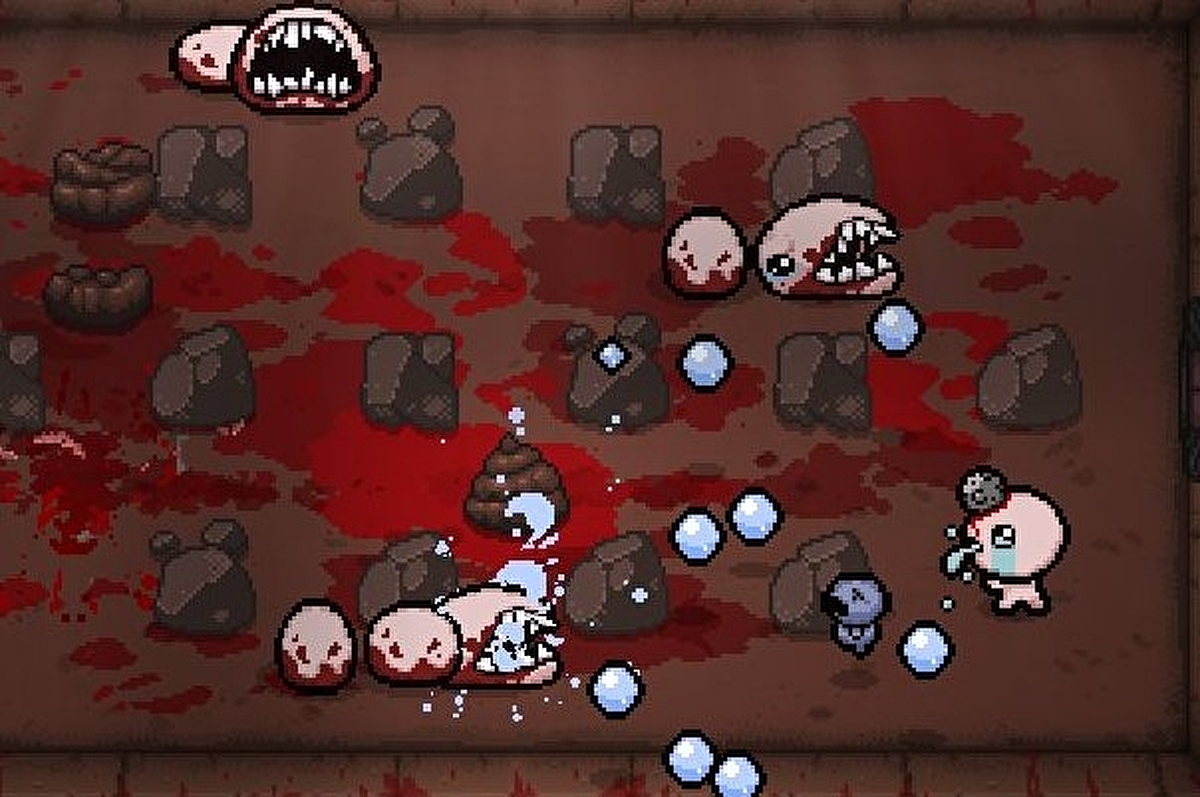
\includegraphics[scale=0.3]{img/The Binding of Isaac.jpg}}
                    \caption{Picture from the binding of Isaac, showing the player (bottom right) attacking the enemies}
                \end{figure}
        \subsection{End Users}
            \subsubsection{\textbf{Description}}
                Teenagers who enjoy exploration video games.
            \subsubsection{Questionnaire}
                \begin{itemize}
                    \item Have you played an exploration game before?
                    \begin{figure}[hbt!]
                        \centerline{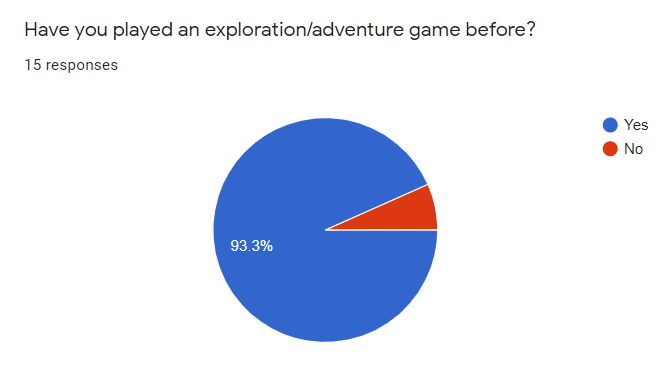
\includegraphics[scale=1]{img/Survey/Played Exploration Game.PNG}}
                        \caption{Responses from survey showing most people have played an exploration game}
                        \label{fig}
                    \end{figure}
                    \clearpage
                    \item How important is each section when looking for a game?
                    \begin{itemize}
                        \item Boss fights
                        \item NPCs that you can interact with
                        \item Enemies that attack you
                        \item Good story
                    \end{itemize}
                    \begin{figure}[hbt!]
                        \centerline{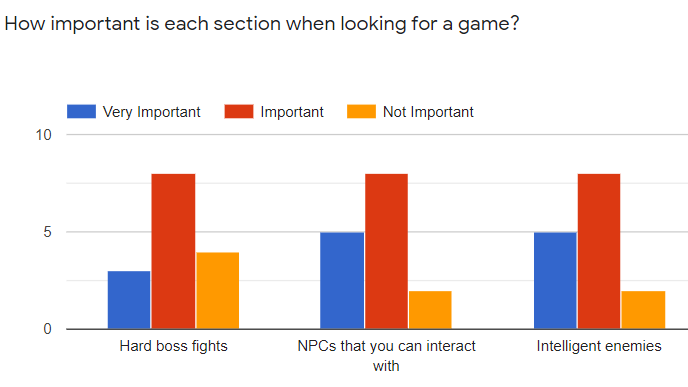
\includegraphics[scale=1]{img/Survey/Importance of games.PNG}}
                        \caption{Responses from the story showing that it is equally important to have intelligent enemies and NPCs you can interact with}
                        \label{fig}
                    \end{figure}
                    \item What era do you like games to be designed as?
                    \begin{itemize}
                        \item Future
                        \item Modern
                        \item Medieval
                        \item Stone Age
                        \item Multiple eras
                    \end{itemize}
                    \begin{figure}[hbt!]
                        \centerline{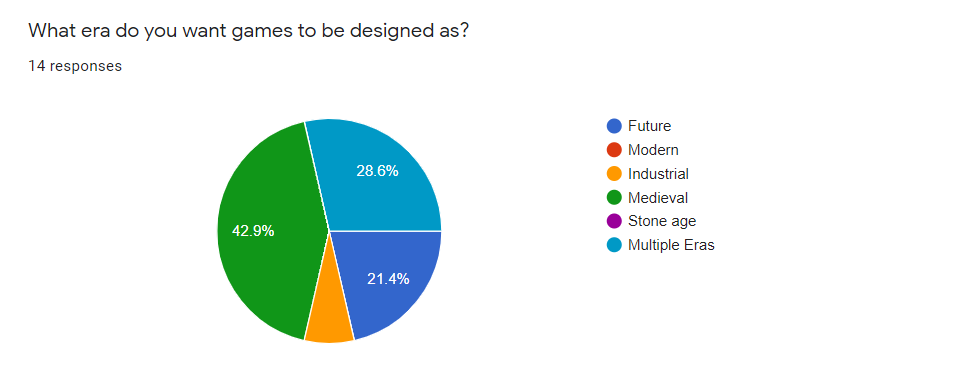
\includegraphics[scale=1]{img/Survey/Era of Games.PNG}}
                        \caption{Responses from survey showing that most people like a Medieval design}
                        \label{fig}
                    \end{figure}
                    \clearpage
                    \item Which do you prefer a weight-based system for the inventory (e.g. in Skyrim) or a space-based system (e.g. Minecraft)?
                    \begin{figure}[hbt!]
                        \centerline{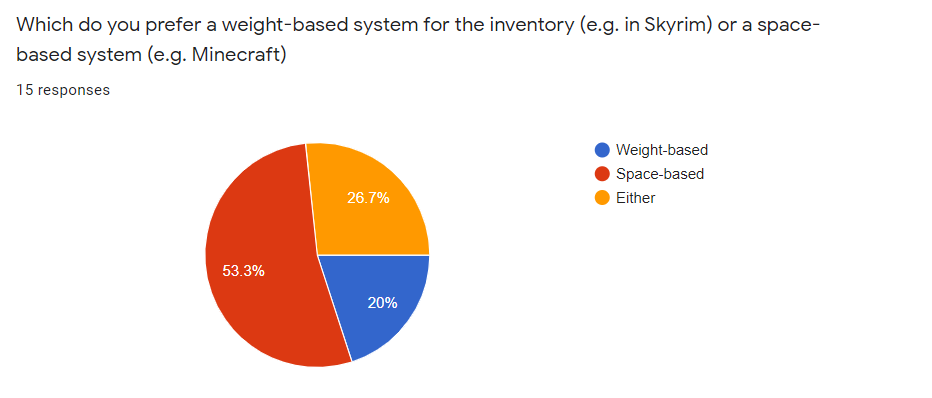
\includegraphics[scale=1]{img/Survey/Inventory system.PNG}}
                        \caption{Responses from survey showing that most people like a weight-based system in a game}
                        \label{fig}
                    \end{figure}
                    \item Do you prefer being able to move while attacking or a Pokémon style attack system?
                    \begin{figure}[hbt!]
                        \centerline{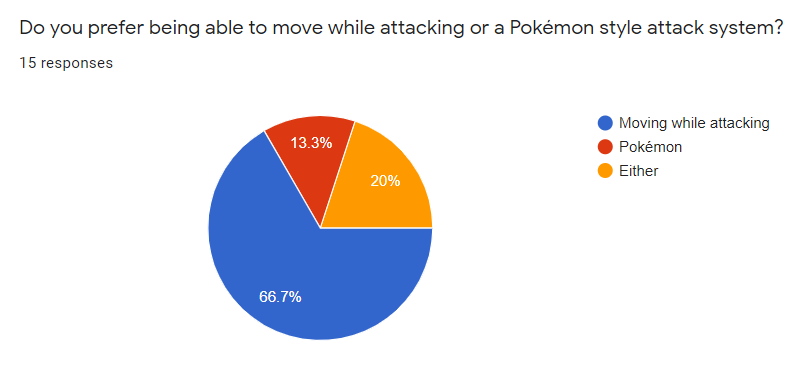
\includegraphics[scale=1]{img/Survey/Attacking System.PNG}}
                        \caption{Responses from survey showing that the attacking system should allow you to still control the player}
                        \label{fig}
                    \end{figure}
                    \clearpage
                    \item Have you played "The Binding of Isaac"?
                    \begin{figure}[hbt!]
                        \centerline{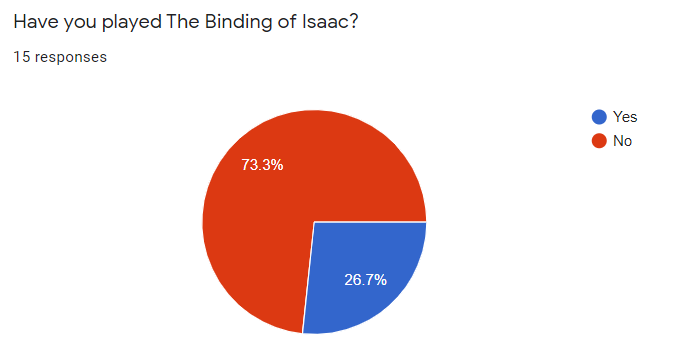
\includegraphics[scale=1]{img/Survey/Capture.PNG}}
                        \caption{Responses from survey showing that most people in this survey had not played The Binding of Isaac}
                        \label{fig}
                    \end{figure}
                    \begin{itemize}
                        \item If they had I asked what they liked about the game and what they think could be better (talked about in the conclusion)
                    \end{itemize}
                \end{itemize}
        \subsubsection{Conclusion}
            As shown in \figurename{ 2}, most people taking the survey had played and exploration or adventure game before, this means that the survey would be somewhat respective of the audience this game will be made for. Surprisingly, in \figurename{ 3}, most people believed that hard boss fights are less important than NPCs you can interact with and intelligent enemies, so I will prioritise those features over creating boss fights. For the design, I will be going for a Medieval theme as it seems as though most people prefer that design scheme (as shown in \figurename{ 4}). Also, I have chosen to use a space-based system for the inventory as in \figurename{ 5}, most people responding that they prefer that system. Also, I will allow the player to attack at any point in the maze (for example shooting a projectile) because (as shown in \figurename{ 6}) people prefer it over an attacking GUI.

            As shown in \figurename{ 7}, only a few percentage had played The Binding of Isaac. when asked what they liked about the game, the responses included:
            \begin{itemize}
                \item The rougelike aspect (a subgenre of game that have generated levels, and tile-based graphics)
                \item The replayability and unique style
            \end{itemize}
            Most responses where talking about the rougelike aspect or the randomised levels. From this I have decided to use tile-based graphics with most sprites with a resolution of 64 pixels by 64 pixels to make it more rougelike also I want to make the maze as randomised as possible, meaning that many stats will be randomised.

            When asked what they would improve about the game, a few people responded saying:
            \begin{itemize}
                \item More routes down
                \item A good run is greatly depend on loot found in the first couple of floors.
            \end{itemize}
            From this, it seems that the reliance of chance for loot needs to be carefully managed. So, to combat this I have decided to change loot up between the levels, meaning that you cannot get overpowered loot on the first levels. Also I have decided to add a leveling system that allows you to upgrade your stats to allow more ways to play the game. Furthermore, I will need to create multiple ways to get down to different levels, for examples stairs, or a hidden passage that leads you to a treasure room on the next level.
        % TODO: Check if there is anything else in which I can have in my analysis
        \clearpage
        \subsection{Objectives}
            \begin{itemize}
                \item Have an effective rendering system
                    \begin{itemize}
                        \item This system must use OpenGL - as it is the graphics library I am using for this project.
                        \item This means having a system in place where I can call a function, giving it a set of values, and then it will be automatically rendered, so that I do not have to deal with keeping track of how much of the buffer is used up
                        \item So once this is complete, I should have be able to render a tile, or multiple tiles on the screen.
                        \item Create a camera class that can move in the 2D plane with the keyboard.
                    \end{itemize}
                \item Be able to generate an infinite maze
                    \begin{itemize}
                        \item This needs the rendering system to be finished, so that I can render the maze once generated.
                        \item The maze needs to be stored in effective means that means that it will not slow down everytime it generates more of the maze.
                        \item This needs to be able to generate a maze from nothing, with most of the board filled up.
                        \item Once this is in place, I can then make is so that once you can move in each direction and the maze will generate more of itself.
                        \item Create a class for the player, allowing them to be rendered into the maze and have the camera follow the player.
                    \end{itemize}
                \item Create NPCs that rome the maze and can start following you
                    \begin{itemize}
                        \item Create a follower class that can be placed and rendered into the world.
                        \item Make it so that the follower can ask the level for the shortest route (which will use the A* algorithm).
                        \item Make it so that once they have the direction they need to go in, that they can move around the map.
                        \item Create each character in the NPCs section, with them stored in the maze level, each of them with a different skin.
                        % \item Alow them to interact with subtitles, so that they can randomly say quotes, with each NPC with their different set of quotes.
                    \end{itemize}
                \item Add items and a way to collect them with a simple space-based inventory system
                    \begin{itemize}
                        \item Add an inventory to each mob (player, follower, enemy)
                        \item Create an item class that can be found in the maze.
                        \item Allow the item to be picked up and put inside the inventory of the player
                        \item Make an inventory system, so that if the player has too much in their inventory they can chose what to get rid of. Implementing a temporary, basic inventory menu.
                        \item Allow items to be parsed to the followers (so that they act like storage for the player)
                    \end{itemize}
                \item Add combat into the game
                    \begin{itemize}
                        \item Add projectile class that can be created by the player and rendered onto the map.
                        \item Allow the projectile to move in the direction the player is facing, and when it collides with an entity or solid tile, it will delete itself.
                        \item Add a particle system, so that the projectile will produce particles with a solid colour, that will decay over time.
                        \item Add an enemy class that can be rendered onto the maze.
                        \item Add a health and other stats (strength, agility ...) for every mob (player, follower, enemy).
                        \item Make it so that when a projectile hits an entity it deals a random amount of damage (in a given range), and check if the entity has died or not. Create a system to deal with the player's death.
                        \item Create an algorithm for the enemies to attack the player and their followers, also allow the followers to use the same algorithm to attack the enemy
                        \item Allow the enemies to have followers, who also attack the player and their followers.
                        \item Add multiple weapons, which have different damages and effects.
                        \item Add an experience counter, which will allow the player to increase their stats
                    \end{itemize}
                \item Create different rooms that can be found in the maze.
                    \begin{itemize}
                        \item Create the each room and its effects in the "Room" section in the "Design Outline".
                        \item This will include creating a chest that randomly generates items inside, which the player can pick up.
                        \item Update the addRoom function to allow the room to be randomised, adding a random room in the place.
                    \end{itemize}
                \item Create a menu system
                    \begin{itemize}
                        \item Create a layer for handling GUI objects.
                        \item Create button objects that can run a function when clicked.
                        \item Overhaul the inventory menu to work with the new system.
                        \item Make the game updates to be paused when inside a menu.
                        \item Create a main menu, where you can start a new game.
                        \item Allow the user to get back to the main menu while playing the game.
                    \end{itemize}
                \item Finalise everything
                    \begin{itemize}
                        \item Allow the game to be saved and loaded from the main menu (saving them in custom files)
                        \item Add more stats to the mobs, which results in different effects to your damage and the number of followers you can have.
                    \end{itemize}
            \end{itemize}
    \clearpage
    \section{Documented Design}
        \subsection{Overview} % TODO: Talk about how the maze is stored
        \subsection{Maze Generation}
            \subsubsection{Prototype}
            For a prototype of the generation, I decided to write it in python with a room just consisting of being a cross section, this was to make sure that it wasn't too complex, while keeping the basic idea of the generation.
            \begin{figure}[hbt!]
                \centerline{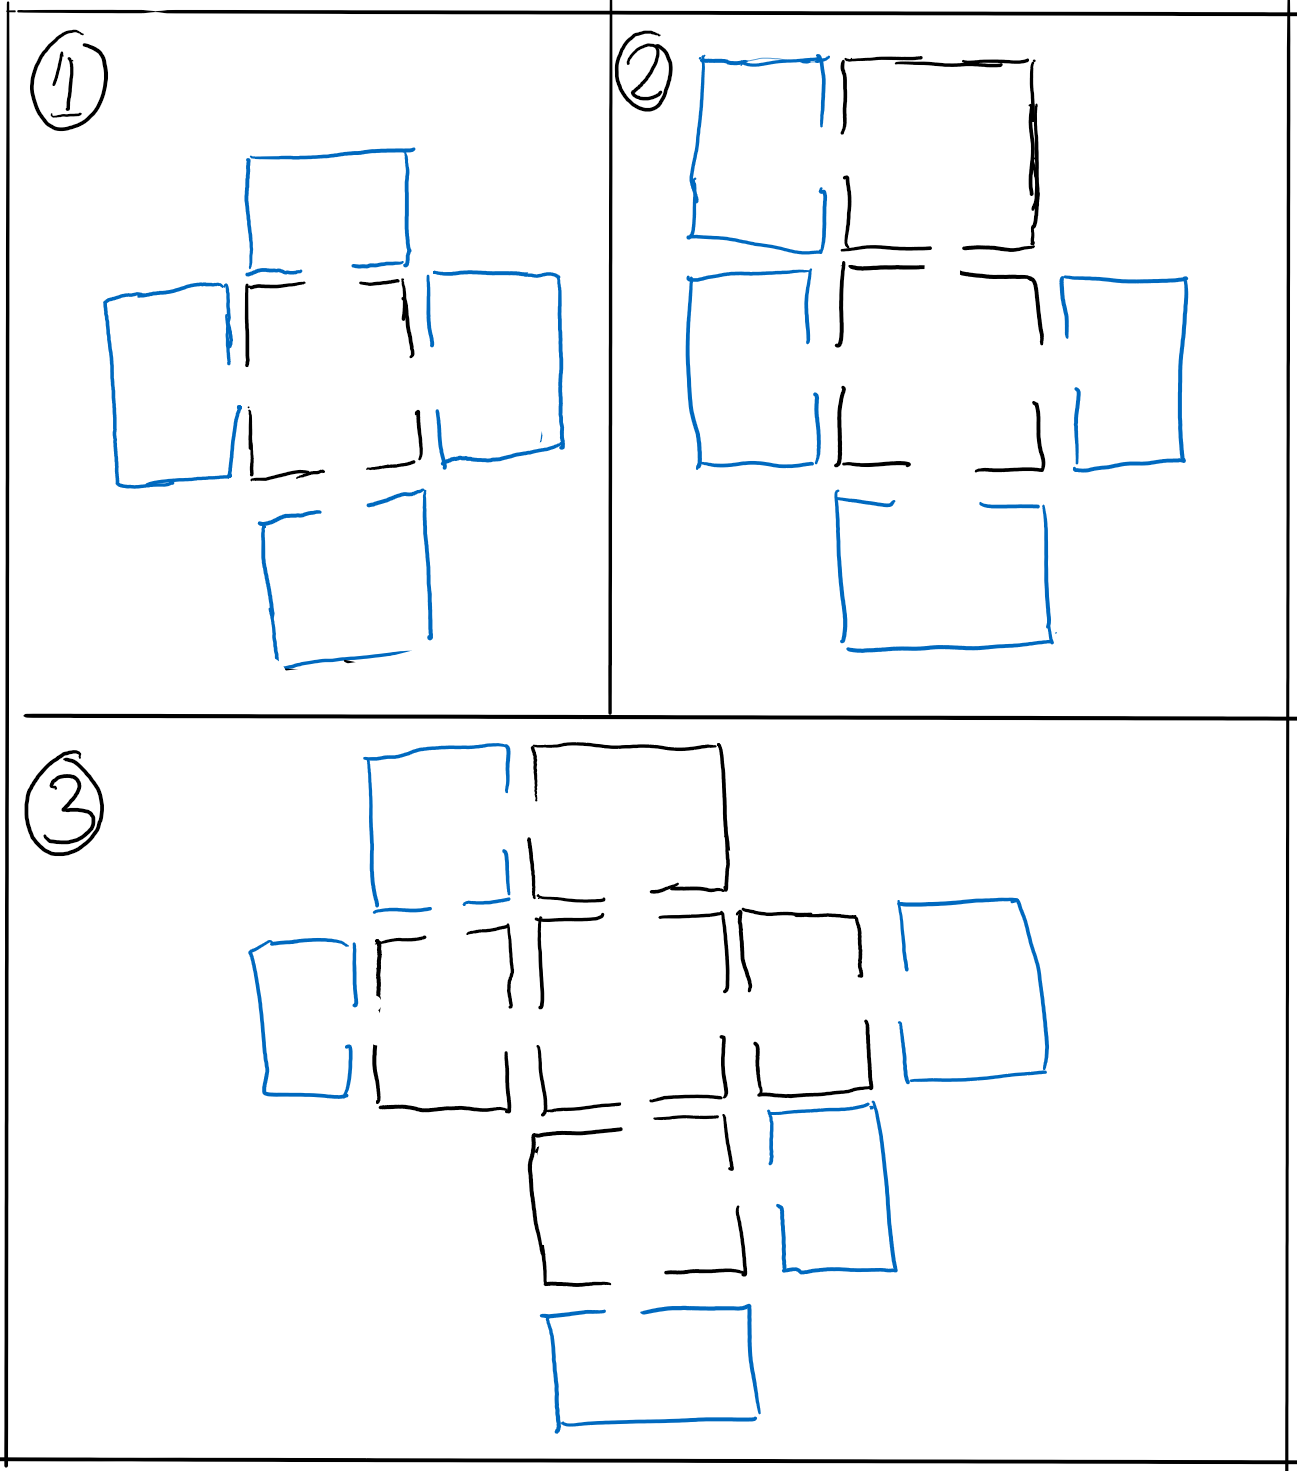
\includegraphics[scale=0.5]{img/Design/Maze Generation.png}}
                \caption{Steps followed by the maze generation}
                \label{fig}
            \end{figure}

            The figure above briefly shows planning behind how the maze generation works, with the rooms outlined in black, as rooms that have a set place, with then the rooms highlighted in blue being the rooms yet to be generated, and thus in the "current" list.

            \clearpage
            \lstinputlisting[language = Python]{prototypes/MazeGen.py}

            \clearpage
            \begin{multicols*}{3}
                [
                    \subsubsection{Output}
                    This is the output of the prototype, with the 'X' representing a wall and blank space represented as path the player can walk through. I have also shown the output of the maze when the player moves south and east. The new sections of the maze generated, after taking each step, is highlighted in yellow.
                ]
                The first output \par
                \centerline{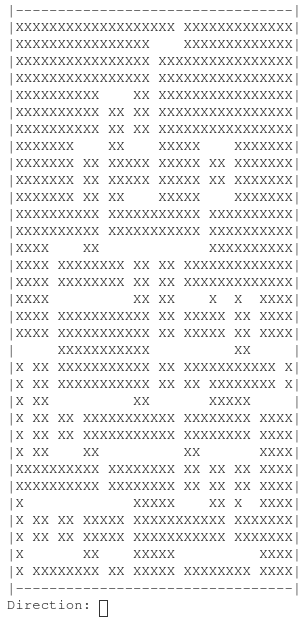
\includegraphics[width=0.8\linewidth]{img/Design/Output1.png}}

                \columnbreak
                After moving south (downwards) \par
                \centerline{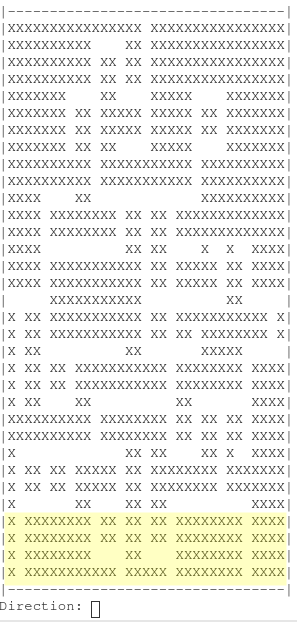
\includegraphics[width=0.75\linewidth]{img/Design/Output2.png}}


                \columnbreak
                After moving east (leftwards) \par
                \centerline{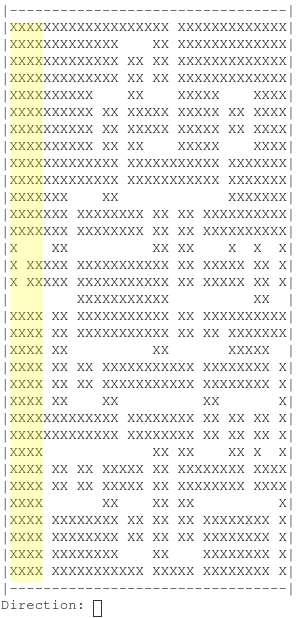
\includegraphics[width=0.8\linewidth]{img/Design/Output3.png}}
            \end{multicols*}

        \subsection{A* Algorithm}
            \subsubsection{Explanation}
                This is a common algorithm used for finding the shortest route between two points because speed while also being very versatile.
                \begin{figure}[hbt!]
                    \centerline{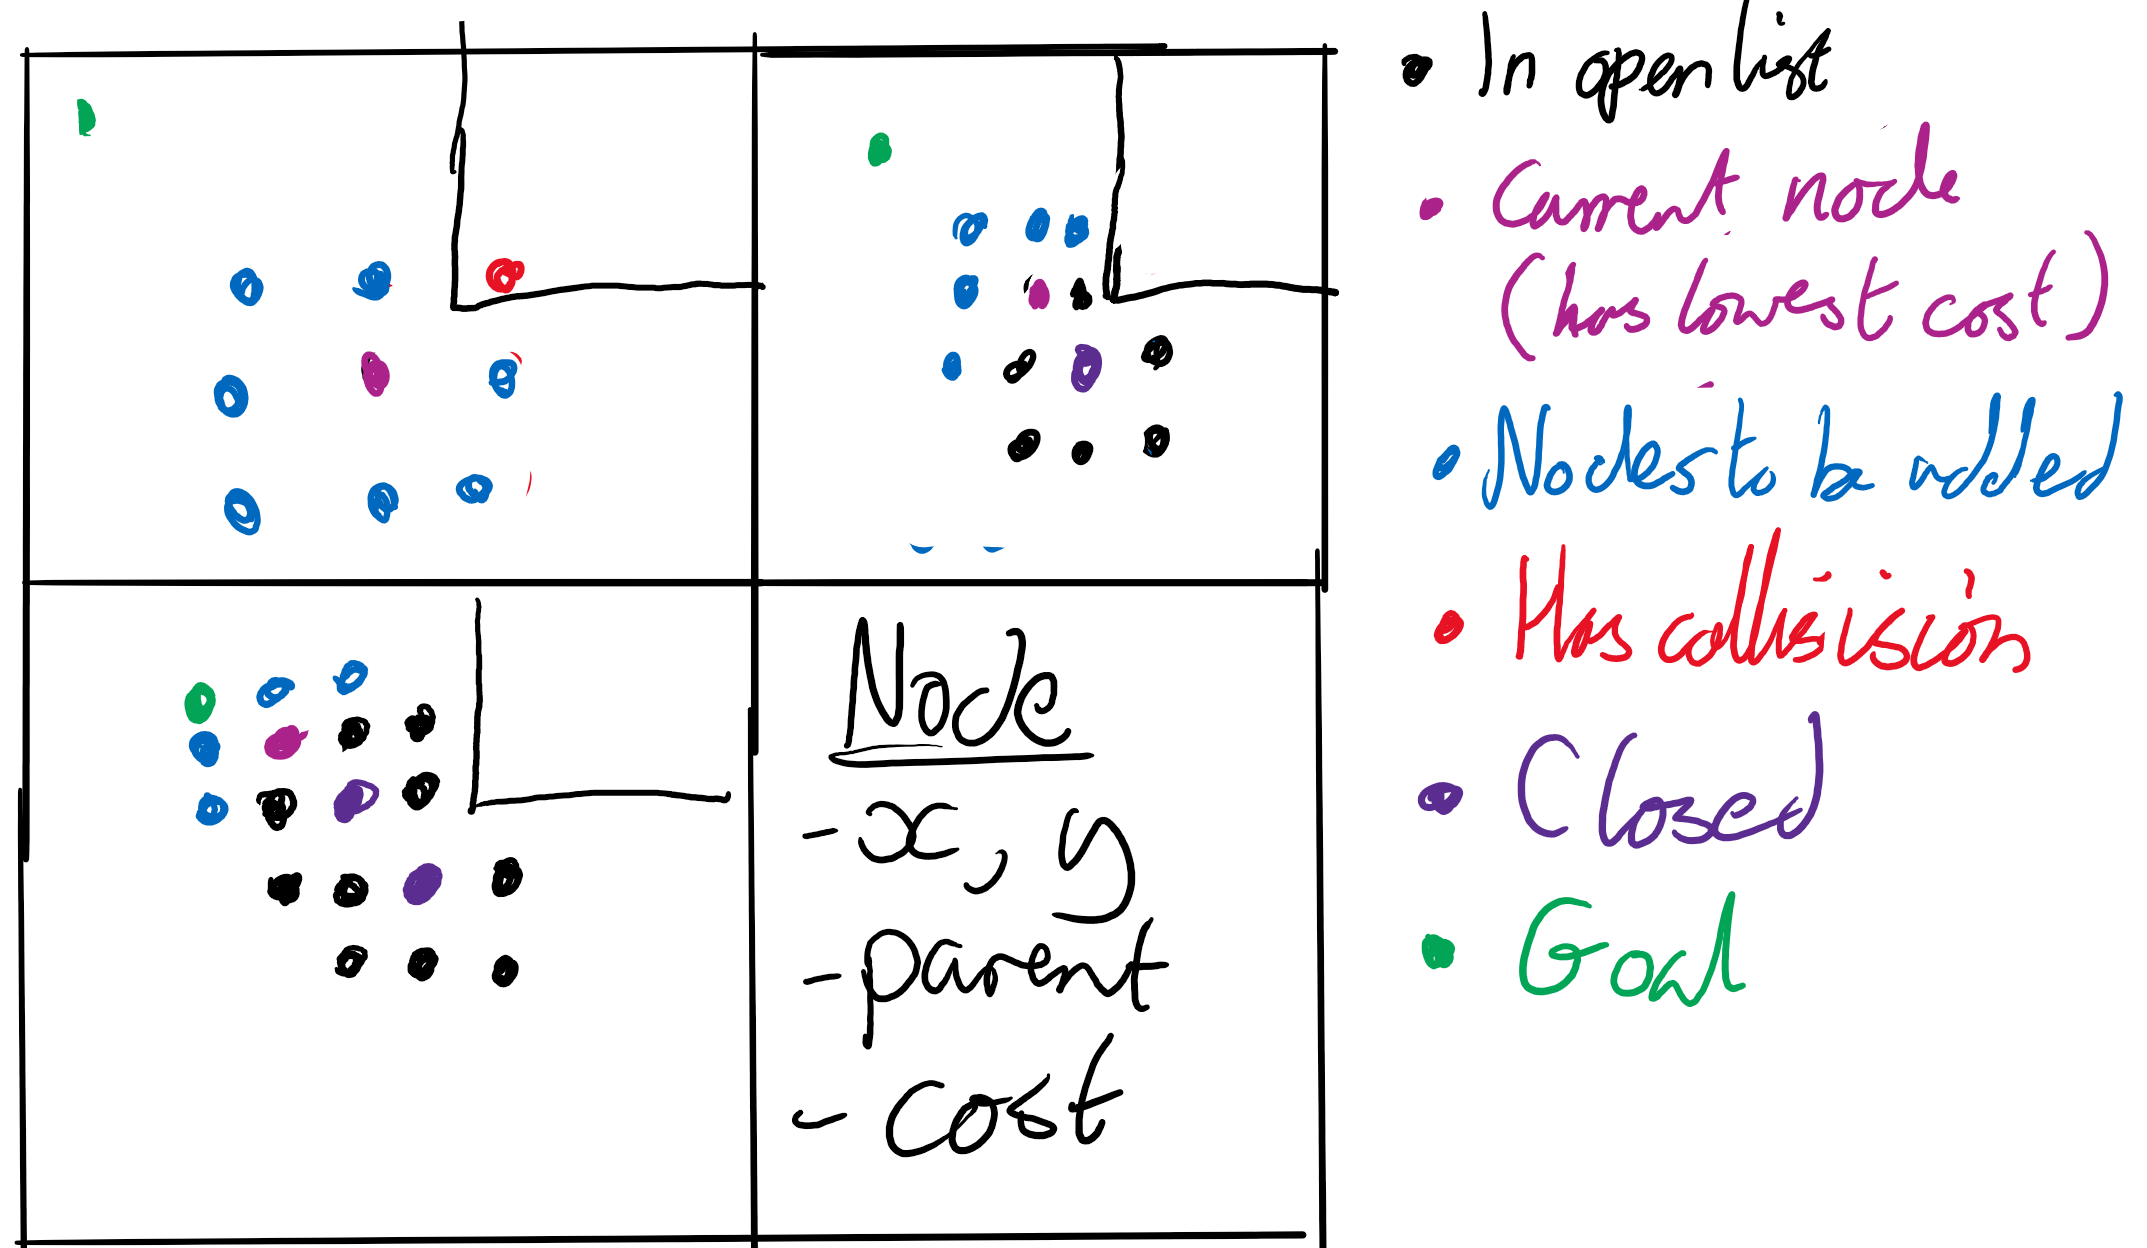
\includegraphics[scale=0.3]{img/Design/A-star algorithm.png}}
                    \caption{Drawing describing the process of how the A* algorithm finds the shortest route}
                    \label{fig}
                \end{figure}

                The final box shows what the Node class needs to store, in order for this to work, with the different colours representing different states a node can be in, labelled on the side.
            \subsubsection{Prototype} % TODO: Write a prototype

        \subsection{Graphical Design}
            \subsubsection{Overall Design}
                The overall design is (as shown below) to have a simple GUI system where the player can see what current weapons they have available to them as well as their health, then a simple button at the top to pause the game and go back to a menu screen. Furthermore, the camera will be facing downwards and is above the player. This will make it easier to create a rendering system and allows the player to explore in any direction (except up and down). Items will be able to be found on the ground, with rendered with their texture, and not a back or anything to allow anyone to easily discern between the different objects.

                Each room will be simple, with different objects in the center, for example this room has a chest in the center which the player will be able to interact with and grab items out of. Then there can be entrances at the top, bottom, left and right of the room and will be generated using the method talked above (in the maze generation section).
                \begin{figure}[hbt!]
                    \centerline{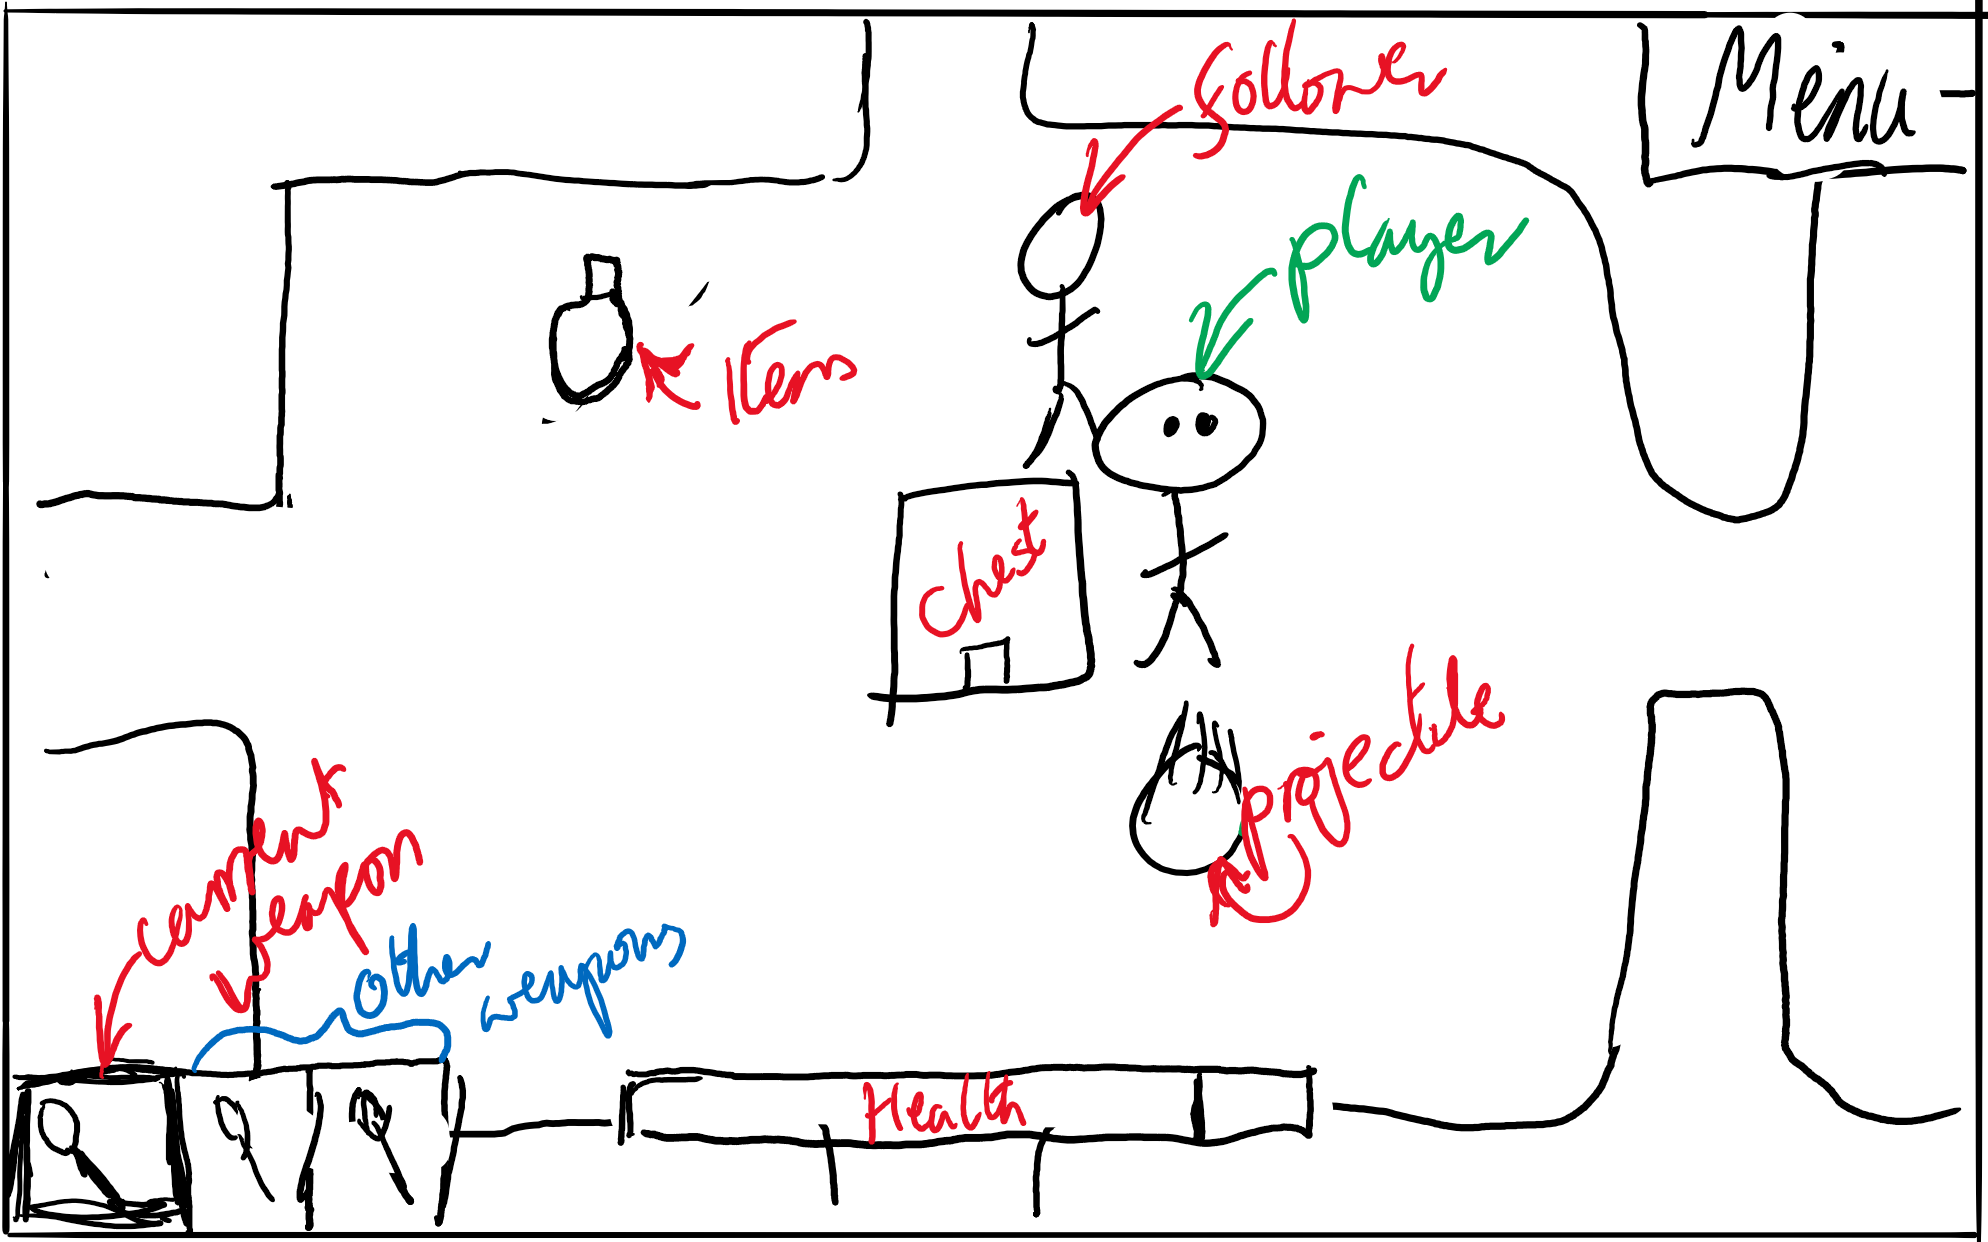
\includegraphics[scale=0.3]{img/Design/Overall Design.png}}
                    \caption{Overall Design plan}
                    \label{fig}
                \end{figure}
            \subsubsection{Characters} % TODO: Update this
            \subsubsection{Enemies}
            \subsubsection{Rooms}

        \subsection{General Design}
            \subsubsection{Stats}
                Each stat will influence part of how you play the game. These will be upgraded through finding specific items in chests and experience gained from doing different activities like exploring or attacking.
                \begin{itemize}
                    \item Strength - Directly effects the damage an entity can do.
                    \item Agility - Increases speed of himself and followers and decreases the speed of attacks.
                    \item Health - Directly effects how long it takes for you to die.
                    \item Combat Ability - Influences the likelihood of higher damages when attacking
                    \item Stamina - Influences the accuracy and damage when attacking and directly influences the amount a mob can carry.
                    \item Boredom - Decreases speed and accuracy. This is decreased through finding items and reading books. This is also contagious between a mob's followers.
                    \item Minimum attack damage - This is damage done when a mob has no weapon.
                    \item Attractiveness - Influences the maximum number of followers each mob can have, however if a mob is following another, this is set to 0.
                \end{itemize}
            \subsubsection{Rooms}
                Each room has their own effects and contains different objects. This will create more variety when exploring.
                \begin{itemize}
                    \item Trap Room - This will contain a trap, which can harm or kill the player or a follower. However, there should also be a chance for the player to avoid the trap through pressing some keys at the right time.
                    \item Treasure Room - This will contain a chest, containing items which the player can collect and distribute to followers.
                    \item Stair Room - This will contain stairs that lead to the next level.
                    \item Trapdoor Room - This can be disguised as a trap room that would cause the player to fall down to the next level.
                    \item Hidden treasure room, this is a room that all the entrances are hidden until the player actively reveals the entrance.
                    \item Enemy room - this should contain an enemy inside the room, which will start attacking when the player walks in. Also the entrances should be closed (this could be the rooms around it entrances closing to create to make sure the player does not get stuck)
                \end{itemize}
        \subsection{Structure Overview}
            \subsubsection{Singletons}
                In the program, there will some key classes that everything will need to have access to. So, to combat this, those classes will be singletons (classes with only one instance ever created). Then these classes will have a get function which will return that single instance and so anything can call it and have access to the functions it needs to. To make this easier, I will also create static versions of each function, which act as a reference to the Implemented function by calling the get function. This will make the code look a lot more readable and thus easier to debug.

                The classes that will be singletons will be:
                \begin{itemize}
                    \item Application - This will control all the layers and store the key information needed for creating a window.
                    \item Render - This will control all the rendering
                    \item Random - This will be the random generator for all the numbers, as in C++ you should only generate a generator once.
                    \item Log - This will be for logging everything to a file and outputting it to the terminal in debug mode
                    \item ShaderEffectsManager - This will control any shader effects that are applied on any layer in the application, storing the effects and handling IDs
                \end{itemize}
            \subsubsection{Layers}
                For rendering and updating, I will be using a layering system, where each layer will have its own effects and control different parts of the game, for example the actual level layer and the GUI layer. This will allow more control over what receives events and what order they get them in, as well has the order in which things are rendered.

                As mentioned above, these layers will be stored by the application function. The application will be in charge of the flow of information and knowing which layers are overlays and which are not.
            \subsubsection{Rendering System}
                For the rendering system, each class that needs to be rendered will have a render function which will be called every frame. This will then call the relevant function in the render class to render itself. These functions should then send the information into a buffer, which then will only be rendered once the appropriate render function is called. This should be automatically called by the Application after each layer. This function will then convert all the information stored on the buffers into vertices which then will be rendered using the correct shader to get the intended effect (This might mean that I have to have multiple buffers for different objects e.g. text and a coloured rectangle)
            \subsubsection{Flow}
                The control of the frame rate and the updates per second will be controlled by a standalone function in the main file. This will make sure the ups (updates per second) will be a continuous 60 ups, while the fps (frames per second) will run as many times per second as possible. This function will call the relevant update and render function in the application class, which will then call the function on every layer. This should mean that everything in any layer is updated and rendered at the correct times.
        \clearpage
        \subsection{Classes}
            \subsubsection{Application}
                \begin{figure}[hbt!]
                    \centerline{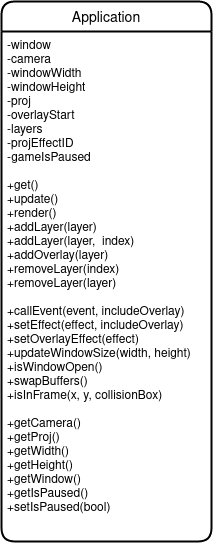
\includegraphics[scale=0.5]{img/Classes/Application.png}}
                    \caption{Application class (singleton)}
                    \label{fig}
                \end{figure}
                \begin{center}
                    Variables
                    \addvbuffer[12pt 8pt]{\begin{tabular}{ | m{0.45\textwidth} | m{0.45\textwidth} | }
                        \hline
                        \textbf{Variable Name} & \textbf{\textbf{Description}} \\
                        \hline
                        window & Stores the application window itself \\
                        \hline
                        camera & Stores the camera that effects the non-overlay layers \\
                        \hline
                        windowWidth & Stores the width of the window \\
                        \hline
                        windowHeight & Stores the height of the window \\
                        \hline
                        proj & Stores the projection map matrix for the window \\
                        \hline
                        overlayStart & Stores the position at which the overlay layers start in the layer stack \\
                        \hline
                        layers & Stores the layer stack \\
                        \hline
                        projEffectID & Stores the ID of the projection effect for all the layers \\
                        \hline
                        gameIsPaused & Stores whether the game is paused or not \\
                        \hline
                    \end{tabular}}

                    \clearpage
                    Functions
                    \begin{tabular}{ | m{0.15\textwidth} | m{0.35\textwidth}| m{0.4\textwidth} | }
                        \hline
                        \textbf{Function Name} & \textbf{Parameters} & \textbf{Description} \\
                        \hline
                        get & & Returns the single instance of the Application \\
                        \hline
                        update & & Calls the update function on all the layers \\
                        \hline
                        render & & Calls the render function on all the layers \\
                        \hline
                        addLayer & Layer you wish to add & Adds a layer to the stack (under the overlays)\\
                        \hline
                        addOverlay & Overlay (as a layer) you wish to add & Adds a layer to the stack on top of all the other layers \\
                        \hline
                        removeLayer & Either the index of the layer or the layer you wish to remove & Removes a layer from the stack \\
                        \hline
                        callEvent & Event and boolean to tell it whether to include the overlay & Calls the event on every layer until one of them uses it \\
                        \hline
                        setEffect & Effect and boolean to tell it whether to include the overlay & Sends the effect to every layer until one of them uses it \\
                        \hline
                        setOverlay & An effect to send & Sends an effect through only the overlays until one of them uses it \\
                        \hline
                        updateWindowSize & The new width and height of the window & Updates the window size stored in the Application \\
                        \hline
                        isWindowOpen & & Returns whether the application is open or not \\
                        \hline
                        swapBuffers & & Swaps the buffers of the application (for rendering) \\
                        \hline
                        isInFrame & x and y of the object and the collision box of the object & Acts as a go between for the camera's isInFrame function \\
                        \hline
                        getCamera & & Returns the camera used for the non-overlay layers \\
                        \hline
                        getProj & & Returns the projection map for the application window \\
                        \hline
                        getWidth & & Returns the width of the application window \\
                        \hline
                        getHeight & & Returns the height of the application window \\
                        \hline
                        getWindow & & Returns the openGL window \\
                        \hline
                        getIsPaused & & Returns whether the game is paused or not (preventing the non-overlay functions from being updated) \\
                        \hline
                        setIsPaused & boolean that the isPaused variable is set to & Sets the isPaused variable \\
                        \hline
                    \end{tabular}
                \end{center}
            \clearpage
            \subsubsection{Render}
                \begin{figure}[hbt!]
                    \centerline{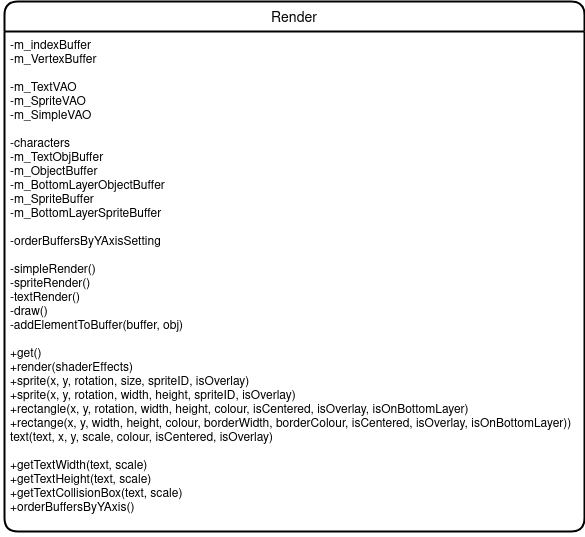
\includegraphics[scale=0.5]{img/Classes/Render.png}}
                    \caption{Render class (singleton)}
                    \label{fig}
                \end{figure}
                \begin{center}
                    Variables
                    \begin{tabular}{ | m{0.45\textwidth} | m{0.45\textwidth} | }
                        \hline
                        \textbf{Variable Name} & \textbf{Description} \\
                        \hline
                        m\_IndexBuffer & Stores the index buffer used for drawing all the vertices in the right order \\
                        \hline
                        m\_VertexBuffer & Stores the buffer used for all the rendering \\
                        \hline
                        m\_TextVAO & Stores the vertex array for drawing text \\
                        \hline
                        m\_SpriteVAO & Stores the vertex array for drawing sprites\\
                        \hline
                        m\_SimpleVAO & Stores the vertex array for drawing rectangles\\
                        \hline
                        characters & Stores all the characters textures and information needed to draw each character of a text font \\
                        \hline
                        m\_TextObjBuffer & Stores all the objects that need to be rendered in this frame \\
                        \hline
                        m\_ObjectBuffer & Stores all the objects that need to be rendered in this frame \\
                        \hline
                        m\_BottomLayerObjectBuffer & Stores all the objects that need to be rendered before anything else on this frame \\
                        \hline
                        m\_SpriteBuffer & Stores all the sprite objects that need to be rendered this frame \\
                        \hline
                        m\_BottomLayerSpriteBuffer & Stores all the sprite objects that need to be rendered before anything else on this frame \\
                        \hline
                        orderBuffersByYAxisSetting & Boolean that tells whether the buffers should be sorted by the Y position of objects \\
                        \hline
                        m\_SpriteShader & Stores the shader for rendering sprites \\
                        \hline
                        m\_TextShader & Stores the shader for rendering text \\
                        \hline
                        m\_SimpleShader & Stores the shader for rendering coloured rectangles \\
                        \hline
                    \end{tabular}
                    Functions
                    \begin{tabular}{ | m{0.2\textwidth} | m{0.3\textwidth}| m{0.4\textwidth} | }
                        \hline
                        \textbf{Function Name} & \textbf{Parameters} & \textbf{Description} \\
                        \hline
                        simpleRender & & Renders everything stored in m\_ObjectBuffer and m\_BottomLayerObjectBuffer \\
                        \hline
                        spriteRender & & Renders everything stored in sprite buffers \\
                        \hline
                        textRender & & Renders everything in m\_TextObjBuffer \\
                        \hline
                        draw & Takes in a VAO to render with & Draws all the vertices stored in m\_VertexBuffer onto the screen with a given VAO \\
                        \hline
                        addElementToBuffer & Takes in the buffer to add the object to and the object & Adds an object onto a buffer taking into account orderBuffersByYAxisSetting \\
                        \hline
                        get & & Returns the only instance of Render \\
                        \hline
                        render & Takes in a list of shaderEffects to apply to the shaders & Sets the shaderEffects to the shaders and then calls the other render functions \\
                        \hline
                        sprite & Takes in all the information needed for rendering (Can use a size or a specific value for the width and the height) & Adds TexturedObject object to the sprite buffers \\
                        \hline
                        rectangle & Takes in all the information to render a rectangle, a second function is made for rendering rectangles with a border & Adds ColouredObject to the object buffers \\
                        \hline
                        text & Takes all the information in to render text on the screen & Adds TextObject to the text buffer\\
                        \hline
                        getTextWidth & Takes in the text and the scale & Returns the width of a given text at a given scale \\
                        \hline
                        getTextHeight & Takes in the text and the scale & Returns the height of the text at a given scale \\
                        \hline
                        getTextCollisionBox & Takes in the text and the scale & Returns the collision box of the text at a given scale \\
                        \hline
                        orderBuffersByYAxis & & Turns the setting on \\
                        \hline
                    \end{tabular}
                \end{center}
            \clearpage
            \subsubsection{Other Singletons}
                \begin{figure}[hbt!]
                    \centerline{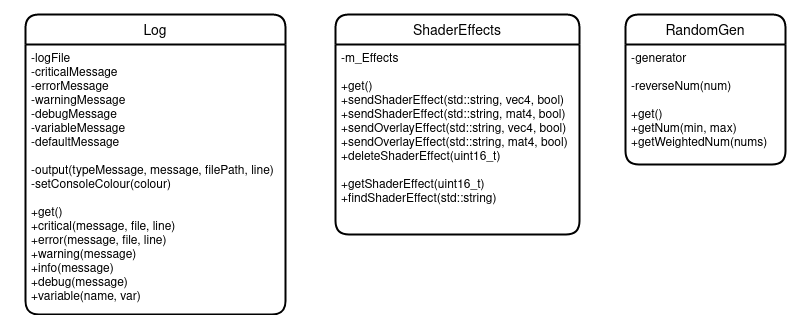
\includegraphics[scale=0.5]{img/Classes/Singletons.png}}
                    \caption{Other singleton classes}
                    \label{fig}
                \end{figure}
                Log
                \begin{center}
                    Variables
                    \begin{tabular}{ | m{0.45\textwidth} | m{0.45\textwidth} | }
                        \hline
                        \textbf{Variable Name} & \textbf{Description} \\
                        \hline
                        logFile & Stores the filename and location of the log file \\
                        \hline
                        criticalMessage & Stores the identifier for a critical message \\
                        \hline
                        errorMessage & Stores the identifier for an error message \\
                        \hline
                        warningMessage & Stores the identifier for a warning message \\
                        \hline
                        debugMessage & Stores the identifier for a debug message \\
                        \hline
                        variableMessage & Stores the identifier for a message with a variable \\
                        \hline
                        defaultMessage & Stores the default identifier \\
                        \hline
                    \end{tabular}
                    Functions
                    \begin{tabular}{ | m{0.15\textwidth} | m{0.35\textwidth}| m{0.4\textwidth} | }
                        \hline
                        \textbf{Function Name} & \textbf{Parameters} & \textbf{Description} \\
                        \hline
                        output & Takes in the identifier and the message as well as the filepath and the line of where the log occurred & Outputs the message in the correct format \\
                        \hline
                        setConsoleColour & A colour & Sets the console to the colour given (in debug mode for the terminal) \\
                        \hline
                        get & & Returns the only instance of the Log class \\
                        \hline
                        critical & Takes in the message and information for debugging & Uses the output function to output a critical message \\
                        \hline
                        error & Takes in the message and information for debugging & Uses the output function to output an error message \\
                        \hline
                        warning & Takes in the message & Uses the output function to output a warning \\
                        \hline
                        info & Takes in a message & Uses the output function to output a message \\
                        \hline
                        debug & Takes in a message & Uses the output function to output a debug message \\
                        \hline
                        variable & Takes in the name of the variable and the variable & Uses the output function to output a variable \\
                        \hline
                    \end{tabular}
                \end{center}
                ShaderEffectsManager
                \begin{center}
                    Variables
                    \begin{tabular}{ | m{0.45\textwidth} | m{0.45\textwidth} | }
                        \hline
                        \textbf{Variable Name} & \textbf{Description} \\
                        \hline
                        m\_Effects & Stores all the effects that are currently in use in the application \\
                        \hline
                    \end{tabular}
                    Functions
                    \begin{tabular}{ | m{0.15\textwidth} | m{0.35\textwidth}| m{0.4\textwidth} | }
                        \hline
                        \textbf{Function Name} & \textbf{Parameters} & \textbf{Description} \\
                        \hline
                        get & & Returns the only instance of the ShaderEffectsManager class \\
                        \hline
                        sendShaderEffect & The name of the effect and the effect (in vector or matrix form) and boolean to say whether it should include the overlays & Creates and sends the effects through the layers \\
                        \hline
                        sendOverlayEffect & The name of the effect and the effect (in vector or matrix form) & Creates and sends an effect through only the overlay layers \\
                        \hline
                        deleteShaderEffect & The ID of the effect & Deletes the effect and sends a message to all the layers to inform them that effect has been deleted \\
                        \hline
                        getShaderEffect & the ID of the effect & Returns the effect associated with that ID \\
                        \hline
                        findShaderEffect & the name of the effect & Finds and returns the ID of the effect with that variable name \\
                        \hline
                    \end{tabular}
                \end{center}
                RandomGen
                \begin{center}
                    Variables
                    \begin{tabular}{ | m{0.45\textwidth} | m{0.45\textwidth} | }
                        \hline
                        \textbf{Variable Name} & \textbf{Description} \\
                        \hline
                        generator & Stores the generator used for all the random number generating (as described in the C++ documentation this should only be created once for each program) \\
                        \hline
                    \end{tabular}
                    Functions
                    \begin{tabular}{ | m{0.15\textwidth} | m{0.35\textwidth}| m{0.4\textwidth} | }
                        \hline
                        \textbf{Function Name} & \textbf{Parameters} & \textbf{Description} \\
                        \hline
                        reverseNum & a number & Returns the number in reverse, used for generating the generator \\
                        \hline
                        get & & Returns the only instance of the RandomGen class \\
                        \hline
                        getNum & Range for the random number & Returns a random number within the range \\
                        \hline
                        getWeightedNum & list of probabilities (should all add up to one) & Returns a random index of the list \\
                        \hline
                    \end{tabular}
                \end{center}
            \clearpage
            \subsubsection{Layers}
                \begin{figure}[hbt!]
                    \centerline{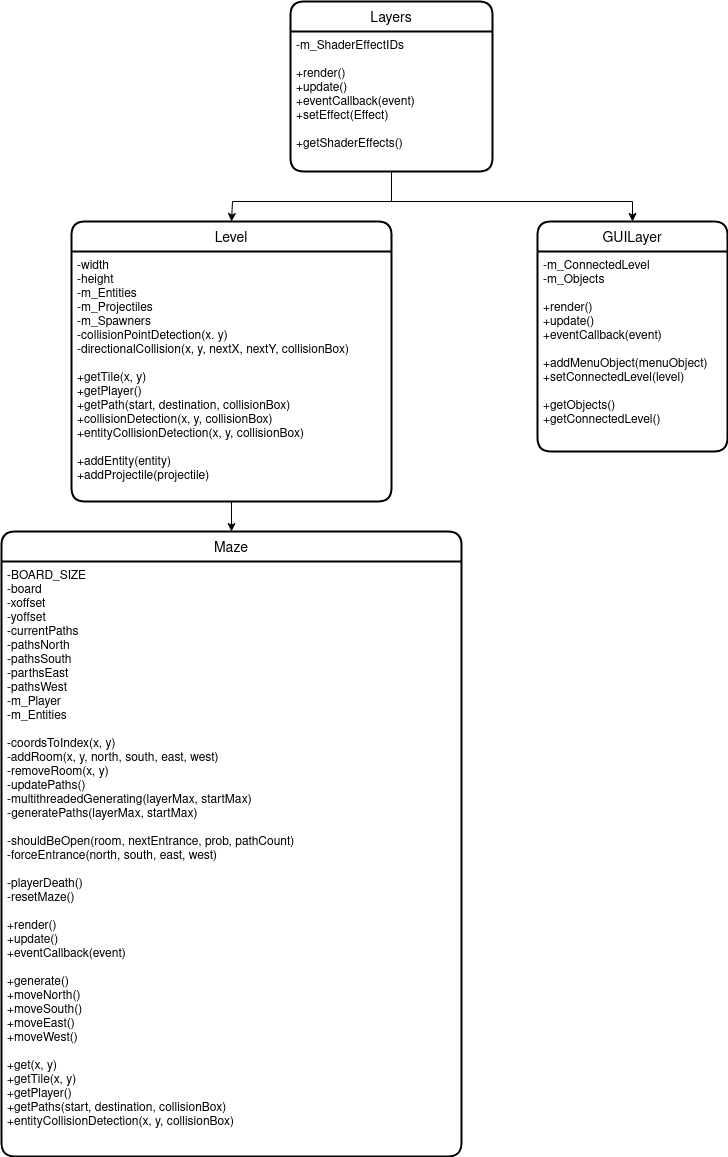
\includegraphics[scale=0.5]{img/Classes/Layers.png}}
                    \caption{Layer subclasses}
                    \label{fig}
                \end{figure}
                Layers
                \begin{center}
                    Variables
                    \begin{tabular}{ | m{0.45\textwidth} | m{0.45\textwidth} | }
                        \hline
                        \textbf{Variable Name} & \textbf{Description} \\
                        \hline
                        m\_ShaderEffectIDs & Stores the effects the layer needs when rendering \\
                        \hline
                    \end{tabular}
                    Functions
                    \begin{tabular}{ | m{0.15\textwidth} | m{0.35\textwidth}| m{0.4\textwidth} | }
                        \hline
                        \textbf{Function Name} & \textbf{Parameters} & \textbf{Description} \\
                        \hline
                        render & & Renders the layer \\
                        \hline
                        update & & Updates the layer \\
                        \hline
                        eventCallback & event that has happened & Allows the layer to interact with events \\
                        \hline
                        setEffect & effect & Sets an effect onto the layer (Will probably be an effect for the shader) \\
                        \hline
                        getShaderEffects & & Returns the shader effects for the layer \\
                        \hline
                    \end{tabular}
                \end{center}
                GUILayer
                \begin{center}
                    Variables
                    \begin{tabular}{ | m{0.45\textwidth} | m{0.45\textwidth} | }
                        \hline
                        \textbf{Variable Name} & \textbf{Description} \\
                        \hline
                        m\_ConnectedLevel & Stores the level it is connected to \\
                        \hline
                        m\_Objects & Stores the objects that are involved in the menu \\
                        \hline
                    \end{tabular}
                    Functions
                    \begin{tabular}{ | m{0.15\textwidth} | m{0.35\textwidth}| m{0.4\textwidth} | }
                        \hline
                        \textbf{Function Name} & \textbf{Parameters} & \textbf{Description} \\
                        \hline
                        addMenuObject & MenuObject to add & Adds a given menu object to the list of objects \\
                        \hline
                        setConnectedLevel & Level to connect to & Connects the layer to a given level (this does not need  to be set - only for menus interacting with the game) \\
                        \hline
                        getObjects & & Returns the list of objects that are involved in the menu \\
                        \hline
                        getConnectedLevel & & Returns the level the layer is connected to \\
                        \hline
                    \end{tabular}
                \end{center}
                Level
                \begin{center}
                    Variables
                    \begin{tabular}{ | m{0.45\textwidth} | m{0.45\textwidth} | }
                        \hline
                        \textbf{Variable Name} & \textbf{Description} \\
                        \hline
                        m\_Player & Stores the player on that level \\
                        \hline
                        width & Stores the width of the level (in terms of tiles)\\
                        \hline
                        height & Stores the height of the level (in terms of tiles)\\
                        \hline
                        m\_Entities & Stores a list of all the entities in the level \\
                        \hline
                        m\_Projectiles & Stores all the projectiles in the level \\
                        \hline
                        m\_Spawners & Stores all the current spawners in the level \\
                        \hline
                    \end{tabular}
                    Functions
                    \begin{tabular}{ | m{0.2\textwidth} | m{0.3\textwidth}| m{0.4\textwidth} | }
                        \hline
                        \textbf{Function Name} & \textbf{Parameters} & \textbf{Description} \\
                        \hline
                        collisionPointDetection & x and y of a point & Calculates whether a point is within a solid tile \\
                        \hline
                        directionalCollision & current x and y and the next x and y and the collision box of the object & Calculates whether an object is going to collide with any tile within the level \\
                        \hline
                        getTile & Tile x and y position in the level & Returns the tile at that point in time \\
                        \hline
                        getPlayer & & Returns the player \\
                        \hline
                        getPath & start position, end position and the collisionBox of the object & Returns a path of the shortest route between two points (using A* algorithm)\\
                        \hline
                        collisionDetection & x, y and collisionBox of an object & returns whether it has collided with anything \\
                        \hline
                        entityCollisionDetection & x, y and collisionBox of an object & returns whether it has collided with an entity in the level \\
                        \hline
                        addEntity & entity & Adds an entity to the level \\
                        \hline
                        addProjectile & projectile & Adds a projectile to the level \\
                        \hline
                        addSpawner & spawner & Adds a spawner to the level \\
                        \hline
                    \end{tabular}
                \end{center}
                Maze
                \begin{center}
                    Variables
                    \begin{tabular}{ | m{0.45\textwidth} | m{0.45\textwidth} | }
                        \hline
                        \textbf{Variable Name} & \textbf{Description} \\
                        \hline
                        BOARD\_SIZE & Static, constant variable that stores the width of the maze (in rooms) \\
                        \hline
                        board & Stores the list of rooms in the maze \\
                        \hline
                        xoffset & Stores the offset in the x direction for the top left corner of the maze \\
                        \hline
                        yoffset & Stores the offset in the y direction for the top left corner of the maze \\
                        \hline
                        currentPaths & Stores the current available paths the maze can generate in (used for generating the maze)\\
                        \hline
                        pathsNorth & Stores the paths that can be generated when the maze moves north \\
                        \hline
                        pathsSouth & Stores the paths that can be generated when the maze moves south \\
                        \hline
                        pathsEast & Stores the paths that can be generated when the maze moves east \\
                        \hline
                        pathsWest & Stores the paths that can be generated when the maze moves west \\
                        \hline
                    \end{tabular}
                    Functions
                    \begin{tabular}{ | m{0.2\textwidth} | m{0.3\textwidth}| m{0.4\textwidth} | }
                        \hline
                        \textbf{Function Name} & \textbf{Parameters} & \textbf{Description} \\
                        \hline
                        coordsToIndex & x and y position of a room & Converts a 2d coordinates for a room into an index of where it is in the board variable \\
                        \hline
                        addRoom & position and booleans for each entrance it could have & This adds a room at given coordinates, randomising what room it is and adding entities into it \\
                        \hline
                        removeRoom & x and y position of the room & This removes a room from the maze \\
                        \hline
                        updatePaths & & This updates the paths variables by resetting them and looking for new ones \\
                        \hline
                        multithreadedGenerating & The maximum layers for a boosted effect of generating and start maximum probability & This sets up everything needed to have the generating of the maze in another thread \\
                        \hline
                        generatePaths &  The maximum layers for a boosted effect of generating and start maximum probability & This is the function written in the prototype transferred for generating the maze using the currentPaths variable \\
                        \hline
                        shouldBeOpen & room, the next entrance, the probability of the entrance and count of how many entrances are already open & This returns an entrance state and chooses whether the entrance, should be open or closed (or it is closed but it could be opened)\\
                        \hline
                        forceEntrance & reference to the boolean values that store whether the entrance is going to be open or not & This will force an entrance, when the program believes there needs to be another entrance when generating \\
                        \hline
                        playerDeath & & This is the function that handles everything when the player dies \\
                        \hline
                        resetMaze & & This deals with resetting the whole maze \\
                        \hline
                        generate & & This is the function to call to generate a new maze \\
                        \hline
                        moveNorth & & This handles the maze moving to the north (and generates new rooms)\\
                        \hline
                        moveSouth & & This handles the maze moving to the south (and generates new rooms)\\
                        \hline
                        moveEast & & This handles the maze moving to the east (and generates new rooms) \\
                        \hline
                        moveWest & & This handles the maze moving to the west (and generates new rooms)\\
                        \hline
                        get & x and y pos of a room & This returns a room at the given coordinates \\
                        \hline
                    \end{tabular}
                \end{center}
            \clearpage
            \subsubsection{Entities}
                \begin{figure}[hbt!]
                    \centerline{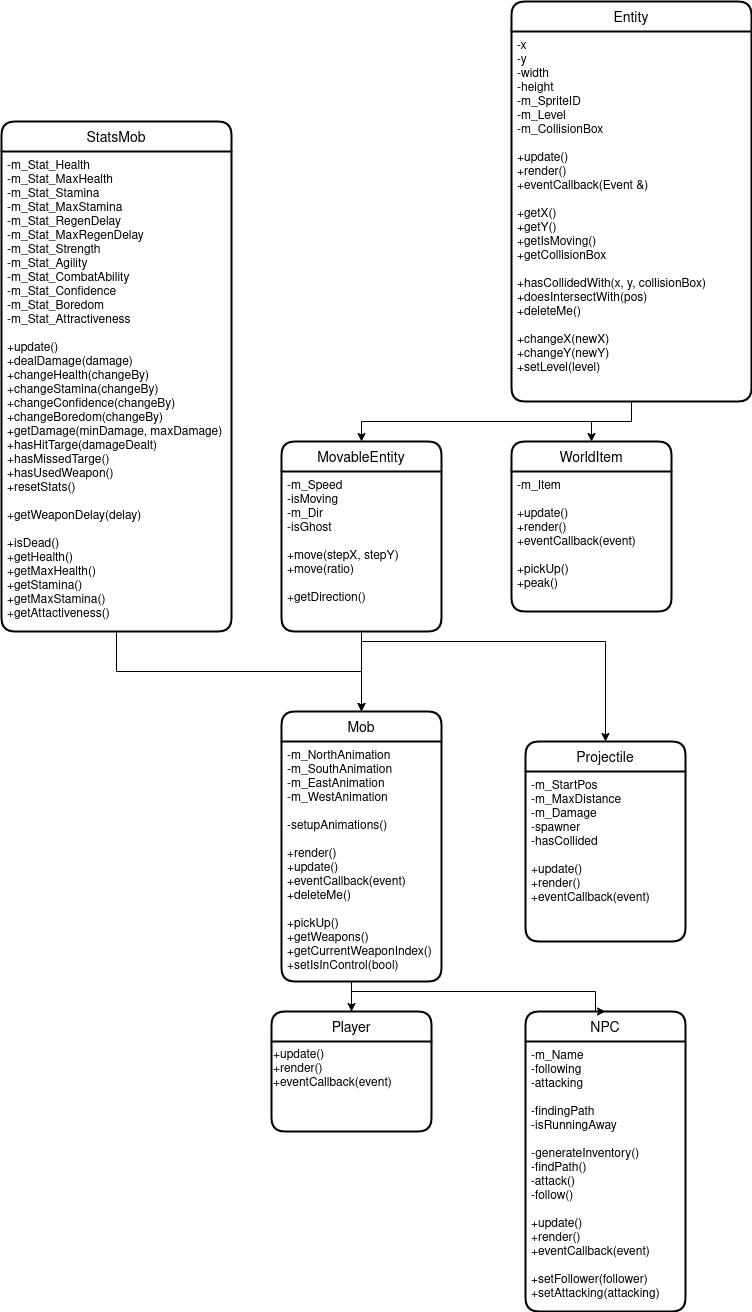
\includegraphics[scale=0.5]{img/Classes/Entities.png}}
                    \caption{Entity subclasses and StatsMob}
                    \label{fig}
                \end{figure}
                Entity
                \begin{center}
                    Variables
                    \begin{tabular}{ | m{0.45\textwidth} | m{0.45\textwidth} | }
                        \hline
                        \textbf{Variable Name} & \textbf{Description} \\
                        \hline
                        x & Stores the x position of the entity \\
                        \hline
                        y & Stores the y position of the entity \\
                        \hline
                        width & Stores the width of the entity \\
                        \hline
                        height & Stores the height of the entity \\
                        \hline
                        m\_SpriteID & Stores the sprite ID of the entity \\
                        \hline
                        m\_Level & Stores the level the entity is located in \\
                        \hline
                        m\_CollisionBox & Stores the collision box of the entity \\
                        \hline
                    \end{tabular}
                    Functions
                    \begin{tabular}{ | m{0.15\textwidth} | m{0.35\textwidth}| m{0.4\textwidth} | }
                        \hline
                        \textbf{Function Name} & \textbf{Parameters} & \textbf{Description} \\
                        \hline
                        update & & Updates the entity \\
                        \hline
                        render & & Renders the entity \\
                        \hline
                        eventCallback & Event & This allows entities to listen for events \\
                        \hline
                        getX & & Returns x position \\
                        \hline
                        getY & & Returns y position \\
                        \hline
                        getIsMoving & & Returns whether the entity is moving \\
                        \hline
                        getCollisionBox & & Returns the collision box \\
                        \hline
                        hasCollidedWith & position and collisionBox of an object & returns whether its collision box intersects with theirs \\
                        \hline
                        doesIntersectWith & position of point & returns whether or not that point is inside its collision box \\
                        \hline
                        deleteMe & & Returns whether the entity should be deleted \\
                        \hline
                        changeX & new x position & changes the x position of the entity \\
                        \hline
                        changeY & new y position & changes the y position of the entity \\
                        \hline
                        setLevel & level the entity is in & changes the level the entity is currently in \\
                        \hline
                    \end{tabular}
                \end{center}
                WorldItem
                \begin{center}
                    Variables
                    \begin{tabular}{ | m{0.45\textwidth} | m{0.45\textwidth} | }
                        \hline
                        \textbf{Variable Name} & \textbf{Description} \\
                        \hline
                        m\_Item & Stores the item that it is carrying \\
                        \hline
                    \end{tabular}
                    Functions
                    \begin{tabular}{ | m{0.15\textwidth} | m{0.35\textwidth}| m{0.4\textwidth} | }
                        \hline
                        \textbf{Function Name} & \textbf{Parameters} & \textbf{Description} \\
                        \hline
                        pickUp & & returns the item and removes it from its storage \\
                        \hline
                        peak & & returns the item however doesn't remove it from its storage \\
                        \hline
                    \end{tabular}
                \end{center}
                MovableEntity
                \begin{center}
                    Variables
                    \begin{tabular}{ | m{0.45\textwidth} | m{0.45\textwidth} | }
                        \hline
                        \textbf{Variable Name} & \textbf{Description} \\
                        \hline
                        m\_Speed & Stores the maximum speed it can travel at \\
                        \hline
                        isMoving & Stores whether it is currently moving or not \\
                        \hline
                        m\_Dir & Stores the direction it is travelling in \\
                        \hline
                        isGhost & Stores whether it ignores collision \\
                        \hline
                    \end{tabular}
                    Functions
                    \begin{tabular}{ | m{0.15\textwidth} | m{0.35\textwidth}| m{0.4\textwidth} | }
                        \hline
                        \textbf{Function Name} & \textbf{Parameters} & \textbf{Description} \\
                        \hline
                        move & Can either be a change in x and y or a ratio (using its maximum speed) & This moves the object, checking for collisions and taking into account its maximum speed \\
                        \hline
                        getDirection & & Returns the current direction of the entity \\
                        \hline
                    \end{tabular}
                \end{center}
                Projectile % TODO: This is incorrect
                \begin{center}
                    Variables
                    \begin{tabular}{ | m{0.45\textwidth} | m{0.45\textwidth} | }
                        \hline
                        \textbf{Variable Name} & \textbf{Description} \\
                        \hline
                        m\_StartPos & Stores the start position of the projectile \\
                        \hline
                        m\_MaxDistance & Stores the maximum distance the projectile can travel before being deleted \\
                        \hline
                        m\_Damage & Stores the maximum damage the projectile can do \\
                        \hline
                        spawner & Stores the Mob who spawned the projectile \\
                        \hline
                        hasCollided & Stores whether it has collided with anything \\
                        \hline
                    \end{tabular}
                \end{center}
                StatsMob
                \begin{center}
                    Variables
                    \begin{tabular}{ | m{0.45\textwidth} | m{0.45\textwidth} | }
                        \hline
                        \textbf{Variable Name} & \textbf{Description} \\
                        \hline
                        m\_Stat\_Health & Stores the health of the mob \\
                        \hline
                        m\_Stat\_MaxHealth & Stores the max health of the mob \\
                        \hline
                        m\_Stat\_Stamina & Stores the stamina of the mob \\
                        \hline
                        m\_Stat\_MaxStamina & Stores the max stamina of the mob \\
                        \hline
                        m\_Stat\_RegenDelay & Acts as a countdown to when the mob can start to regen its stats\\
                        \hline
                        m\_Stat\_MaxRegenDelay & Stores the maximum value of the regen delay counter\\
                        \hline
                        m\_Stat\_Strength & Stores the strength of mob \\
                        \hline
                        m\_Stat\_Agility & Stores the agility of the mob \\
                        \hline
                        m\_Stat\_CombatAbility & Stores the combat ability of the mob \\
                        \hline
                        m\_Stat\_Confidence & Stores the confidence of the mob (out of 100) \\
                        \hline
                        m\_Stat\_Boredom & Stores the boredom of the mob (out of 100) \\
                        \hline
                        m\_Stat\_Attractiveness & Stores the amount of followers the mob can have \\
                        \hline
                    \end{tabular}
                    Functions
                    \begin{tabular}{ | m{0.15\textwidth} | m{0.35\textwidth}| m{0.4\textwidth} | }
                        \hline
                        \textbf{Function Name} & \textbf{Parameters} & \textbf{Description} \\
                        \hline
                        update & & Updates the regen delay and handles regeneration of the mob's stats \\
                        \hline
                        dealDamage & max damage of weapon & Deals damage to the mob, taking into account their stats \\
                        \hline
                        changeHealth & changeBy & Changes the health (ignoring stats) \\
                        \hline
                        changeStamina & changeBy & Changes the stamina \\
                        \hline
                        changeConfidence & changeBy & Changes the confidence \\
                        \hline
                        changeBoredom & changeBy & Changes the boredom \\
                        \hline
                        getDamage & min and max damage of a weapon & Returns the damage the weapon should do taking into account the mob's stats \\
                        \hline
                        hasHitTarget & damage dealt & Increases the stats based on how much damage a weapon did \\
                        \hline
                        hasMissedTarget & & Changes stats for missing the targe \\
                        \hline
                        hasUsedWeapon & & Resets the regen delay (cannot regen while attacking) \\
                        \hline
                        resetStats & & Resets stats \\
                        \hline
                        getWeaponDelay & max delay of weapon & Returns the delay on a weapon taking into account its stats \\
                        \hline
                        isDead & & Returns true if the health is 0 \\
                        \hline
                        getHealth & & Returns the Mob's health \\
                        \hline
                        getMaxHealth & & Returns the max health of the mob \\
                        \hline
                        getStamina & & Returns the stamina of the mob \\
                        \hline
                        getMaxStamina & & Returns the max stamina of the mob \\
                        \hline
                        getAttractiveness & & Returns the attractiveness of a mob \\
                        \hline
                    \end{tabular}
                \end{center}
                Mob
                \begin{center}
                    Variables
                    \begin{tabular}{ | m{0.45\textwidth} | m{0.45\textwidth} | }
                        \hline
                        \textbf{Variable Name} & \textbf{Description} \\
                        \hline
                        m\_NorthAnimation & Stores the animation sprite for walking north \\
                        \hline
                        m\_SouthAnimation & Stores the animation sprite for walking south \\
                        \hline
                        m\_EastAnimation & Stores the animation sprite for walking east \\
                        \hline
                        m\_WestAnimation & Stores the animation sprite for walking west \\
                        \hline
                        m\_Weapons & Stores all the weapons of the mob \\
                        \hline
                        currentWeapon & Stores the current active weapon \\
                        \hline
                        m\_Inventory & Stores the inventory of the mob \\
                        \hline
                        isInControl & States whether the mob is inControl of its actions \\
                        \hline
                    \end{tabular}
                    Functions
                    \begin{tabular}{ | m{0.2\textwidth} | m{0.3\textwidth}| m{0.4\textwidth} | }
                        \hline
                        \textbf{Function Name} & \textbf{Parameters} & \textbf{Description} \\
                        \hline
                        setupAnimations & & Initialises the animations for each direction \\
                        \hline
                        pickUp & Item to pick up & Adds an item into the inventory \\
                        \hline
                        getWeapons & & Returns the weapons \\
                        \hline
                        getCurrentWeaponIndex & & Returns the current weapon index \\
                        \hline
                        getInventory & & Returns the inventory \\
                        \hline
                        setIsInControl & bool & Sets isInControl \\
                        \hline
                    \end{tabular}
                \end{center}
                Player \\
                The player, only overrides classes its parent classes to achieve functionality \\
                NPC
                \begin{center}
                    Variables
                    \begin{tabular}{ | m{0.45\textwidth} | m{0.45\textwidth} | }
                        \hline
                        \textbf{Variable Name} & \textbf{Description} \\
                        \hline
                        m\_Name & Stores the name of the follower/enemy \\
                        \hline
                        following & Stores the entity that it is following \\
                        \hline
                        attacking & Stores the entity that it is attacking \\
                        \hline
                        findingPath & Stores whether it is currently finding a path to take \\
                        \hline
                        isRunningAway & Stores whether it is running away from its enemy \\
                        \hline
                    \end{tabular}
                    Functions
                    \begin{tabular}{ | m{0.15\textwidth} | m{0.35\textwidth}| m{0.4\textwidth} | }
                        \hline
                        \textbf{Function Name} & \textbf{Parameters} & \textbf{Description} \\
                        \hline
                        generateInventory & & Generates the inventory of the NPC \\
                        \hline
                        findPaths & & Finds the quickest route to the entity it is following \\
                        \hline
                        attack & & Runs algorithm for attacking \\
                        \hline
                        follow & & Runs algorithm for following \\
                        \hline
                        setFollower & follower & Sets the entity it is following \\
                        \hline
                        setAttacking & attacking & Sets the entity it is attacking \\
                        \hline
                    \end{tabular}
                \end{center}
            \clearpage
            \subsubsection{Maze objects}
                \begin{figure}[hbt!]
                    \centerline{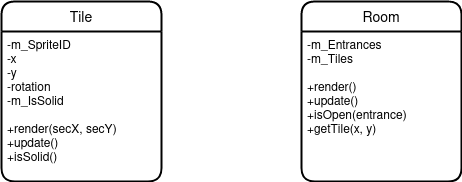
\includegraphics[scale=0.5]{img/Classes/Rooms.png}}
                    \caption{Classes for the design of the maze}
                    \label{fig}
                \end{figure}
                Tile
                \begin{center}
                    Variables
                    \begin{tabular}{ | m{0.45\textwidth} | m{0.45\textwidth} | }
                        \hline
                        \textbf{Variable Name} & \textbf{Description} \\
                        \hline
                        m\_SpriteID & Stores the sprite ID of the tile \\
                        \hline
                        x & Stores the x axis relative to the room it is located in \\
                        \hline
                        y & Stores the y axis relative to the room it is located in \\
                        \hline
                        rotation & Stores the rotation of the tile \\
                        \hline
                        m\_IsSolid & Stores whether it is solid or not \\
                        \hline
                    \end{tabular}
                    Functions
                    \begin{tabular}{ | m{0.15\textwidth} | m{0.35\textwidth}| m{0.4\textwidth} | }
                        \hline
                        \textbf{Function Name} & \textbf{Parameters} & \textbf{Description} \\
                        \hline
                        render & The x and y coordinates of the room it is in & Renders the tile \\
                        \hline
                        update & & Updates the tile (This is not really used as I do not have any animated tiles) \\
                        \hline
                        isSolid & & Returns m\_IsSolid \\
                        \hline
                    \end{tabular}
                \end{center}
                Room
                \begin{center}
                    Variables
                    \begin{tabular}{ | m{0.45\textwidth} | m{0.45\textwidth} | }
                        \hline
                        \textbf{Variable Name} & \textbf{Description} \\
                        \hline
                        m\_Entrances & Stores the entrances and whether they are open or not\\
                        \hline
                        m\_Tiles & Stores all the tiles as a grid \\
                        \hline
                    \end{tabular}
                    Functions
                    \begin{tabular}{ | m{0.15\textwidth} | m{0.35\textwidth}| m{0.4\textwidth} | }
                        \hline
                        \textbf{Function Name} & \textbf{Parameters} & \textbf{Description} \\
                        \hline
                        render & & Renders all the tiles \\
                        \hline
                        update & & Updates the room \\
                        \hline
                        isOpen & Entrance (this is its own type) & returns whether an entrance is open \\
                        \hline
                        getTile & x and y position & Returns a tile at the give coordinates \\
                        \hline
                    \end{tabular}
                \end{center}
            \clearpage
            \subsubsection{Rendering Utils}
                \begin{figure}[hbt!]
                    \centerline{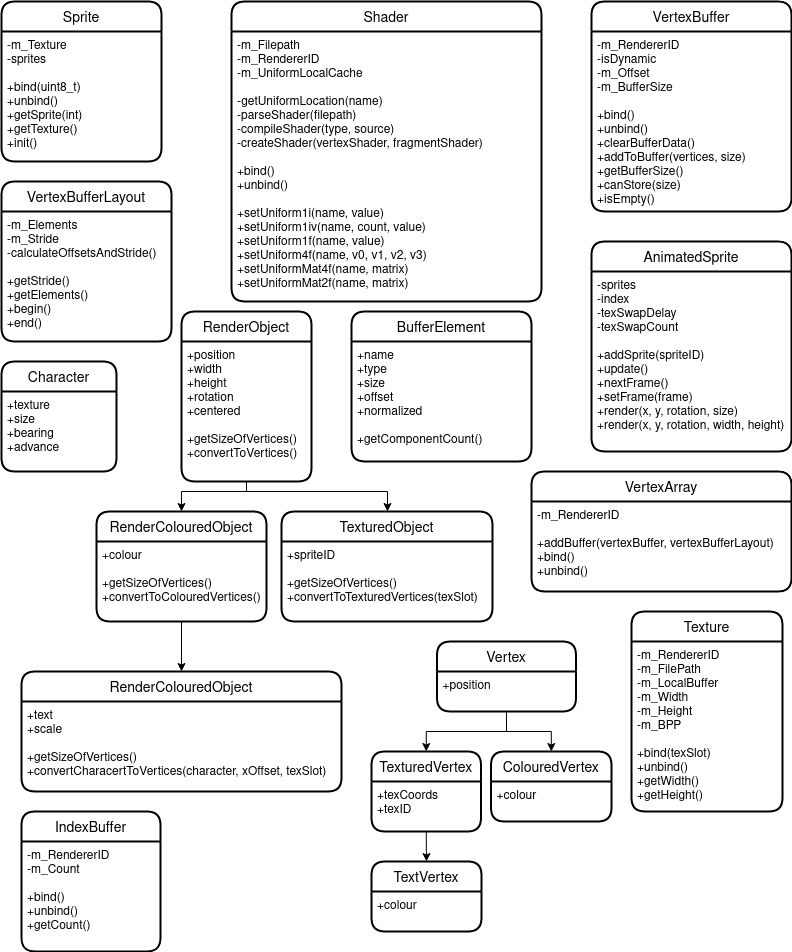
\includegraphics[scale=0.5]{img/Classes/Rendering Utils.png}}
                    \caption{Classes involved in rendering}
                    \label{fig}
                \end{figure}
                Sprite
                \begin{center}
                    Variables
                    \begin{tabular}{ | m{0.45\textwidth} | m{0.45\textwidth} | }
                        \hline
                        \textbf{Variable Name} & \textbf{Description} \\
                        \hline
                        m\_Texture & Stores the texture for that sprite \\
                        \hline
                        sprites & Array that stores all the current sprites in the program \\
                        \hline
                    \end{tabular}
                    Functions
                    \begin{tabular}{ | m{0.15\textwidth} | m{0.35\textwidth}| m{0.4\textwidth} | }
                        \hline
                        \textbf{Function Name} & \textbf{Parameters} & \textbf{Description} \\
                        \hline
                        bind & Slot ID & Binds the texture at a given slot \\
                        \hline
                        unbind & & Unbinds a given its texture \\
                        \hline
                        getSprite & Sprite ID & returns a sprite in the list \\
                        \hline
                        getTexture & & Returns its texture \\
                        \hline
                        init & & Run at the start of the program to initialise all the sprites \\
                        \hline
                    \end{tabular}
                \end{center}
                Shader
                \begin{center}
                    Variables
                    \begin{tabular}{ | m{0.45\textwidth} | m{0.45\textwidth} | }
                        \hline
                        \textbf{Variable Name} & \textbf{Description} \\
                        \hline
                        m\_Filepath & Used for debugging - Stores the filepath of the shader \\
                        \hline
                        m\_RenderID & openGL ID used for interactions with the shader \\
                        \hline
                        m\_UniformLocalCache & Stores all the locations of the uniforms in the shader for quick access \\
                        \hline
                    \end{tabular}
                    Functions
                    \begin{tabular}{ | m{0.15\textwidth} | m{0.35\textwidth}| m{0.4\textwidth} | }
                        \hline
                        \textbf{Function Name} & \textbf{Parameters} & \textbf{Description} \\
                        \hline
                        getUniformLocation & name of the variable & returns the location of the variable in the shader \\
                        \hline
                        parseShader & filepath to the shader & returns vertex and buffer shader from the filepath \\
                        \hline
                        compileShader & type of shader and the source of the shader & compiles the shader and returns ID \\
                        \hline
                        createShader & vertex and fragment shader code & compiles and links the shader \\
                        \hline
                        bind & & Binds the shader \\
                        \hline
                        unbind & & Unbinds the shader \\
                        \hline
                        setUniform1i & name of the variable and the integer & Attaches the value to the uniform \\
                        \hline
                        setUniform1iv & name of the variable and how many is in the list, then pointer to first element & Attaches the value to the uniform \\
                        \hline
                        setUniform1f & name of the variable then the float & Attaches the value to the uniform \\
                        \hline
                        setUniform4f & name of the variable then the four floats & Attaches the value to the uniform \\
                        \hline
                        setUniformMat4f & name and then the matrix & Attaches the value to the uniform \\
                        \hline
                        setUniformMat2f & name and then the matrix & Attaches the value to the uniform \\
                        \hline
                    \end{tabular}
                \end{center}
                VertexBufferLayout
                \begin{center}
                    Variables
                    \begin{tabular}{ | m{0.45\textwidth} | m{0.45\textwidth} | }
                        \hline
                        \textbf{Variable Name} & \textbf{Description} \\
                        \hline
                        m\_Elements & Stores the elements of the layout \\
                        \hline
                        m\_Stride & Stores the length of how long each vertex is \\
                        \hline
                    \end{tabular}
                    Functions
                    \begin{tabular}{ | m{0.2\textwidth} | m{0.3\textwidth}| m{0.4\textwidth} | }
                        \hline
                        \textbf{Function Name} & \textbf{Parameters} & \textbf{Description} \\
                        \hline
                        calculateOffsetsAndStride & & Calculates all the offsets for the elements \\
                        \hline
                        getStride & & Returns the stride \\
                        \hline
                        getElements & & Returns the elements \\
                        \hline
                        begin & & Go between function for the vector m\_Elements \\
                        \hline
                        end & & Go between function for the vector m\_Elements \\
                        \hline
                    \end{tabular}
                \end{center}
                Character
                \begin{center}
                    Variables
                    \begin{tabular}{ | m{0.45\textwidth} | m{0.45\textwidth} | }
                        \hline
                        \textbf{Variable Name} & \textbf{Description} \\
                        \hline
                        texture & Stores the texture for the character \\
                        \hline
                        size & A vector that stores the width and height of the character \\
                        \hline
                        bearing & A vector that stores the position relative to the origin \\
                        \hline
                        advance & Stores the position of the next character relative to itself\\
                        \hline
                    \end{tabular}
                \end{center}
                BufferElement
                \begin{center}
                    Variables
                    \begin{tabular}{ | m{0.45\textwidth} | m{0.45\textwidth} | }
                        \hline
                        \textbf{Variable Name} & \textbf{Description} \\
                        \hline
                        name & Stores the name of the variable input \\
                        \hline
                        type & Stores the type of the variable \\
                        \hline
                        size & Stores the size of the variable \\
                        \hline
                        offset & Stores the offset of its start position \\
                        \hline
                        normalized & Stores whether it is normalized \\
                        \hline
                    \end{tabular}
                    Functions
                    \begin{tabular}{ | m{0.15\textwidth} | m{0.35\textwidth}| m{0.4\textwidth} | }
                        \hline
                        \textbf{Function Name} & \textbf{Parameters} & \textbf{Description} \\
                        \hline
                        getCompoundCount & & Returns the count of elements in each type \\
                        \hline
                    \end{tabular}
                \end{center}
                VertexBuffer
                \begin{center}
                    Variables
                    \begin{tabular}{ | m{0.45\textwidth} | m{0.45\textwidth} | }
                        \hline
                        \textbf{Variable Name} & \textbf{Description} \\
                        \hline
                        m\_RendererID & Stores the ID of the buffer \\
                        \hline
                        m\_Offset & Stores the current offset of the buffer of inputting elements \\
                        \hline
                        m\_BufferSize & Stores the buffer size \\
                        \hline
                    \end{tabular}
                    Functions
                    \begin{tabular}{ | m{0.15\textwidth} | m{0.35\textwidth}| m{0.4\textwidth} | }
                        \hline
                        \textbf{Function Name} & \textbf{Parameters} & \textbf{Description} \\
                        \hline
                        bind & & Binds the buffer \\
                        \hline
                        unbind & & Unbinds the buffer \\
                        \hline
                        clearBufferData & & Clears all the data on the buffer \\
                        \hline
                        addToBuffer & pointer to the vertices and the size of the vertices & Adds data to the buffer \\
                        \hline
                        getBufferSize & & Returns the buffer size \\
                        \hline
                        canStore & Size of the data & Checks to see if it can store that data size \\
                        \hline
                        isEmpty & & Returns if the buffer is empty \\
                        \hline
                    \end{tabular}
                \end{center}
                AnimatedSprite
                \begin{center}
                    Variables
                    \begin{tabular}{ | m{0.45\textwidth} | m{0.45\textwidth} | }
                        \hline
                        \textbf{Variable Name} & \textbf{Description} \\
                        \hline
                        sprites & Stores all the sprite IDs \\
                        \hline
                        index & Stores the current index of the sprite it is on \\
                        \hline
                        texSwapDelay & Stores the delay between the animations \\
                        \hline
                        texSwapCount & Stores the counter for the update cycles between the increasing of the index \\
                        \hline
                    \end{tabular}
                    Functions
                    \begin{tabular}{ | m{0.15\textwidth} | m{0.35\textwidth}| m{0.4\textwidth} | }
                        \hline
                        \textbf{Function Name} & \textbf{Parameters} & \textbf{Description} \\
                        \hline
                        addSprite & sprite ID & Adds the sprite onto the animation \\
                        \hline
                        update & & Increases the count and goes to next sprite if needed \\
                        \hline
                        nextFrame & & Increases index by one \\
                        \hline
                        setFrame & frame index & Sets the frame to the input \\
                        \hline
                        render & Coords and rotation and either width and height or size & Renders the current sprite active \\
                        \hline
                    \end{tabular}
                \end{center}
                VertexArray
                \begin{center}
                    Variables
                    \begin{tabular}{ | m{0.45\textwidth} | m{0.45\textwidth} | }
                        \hline
                        \textbf{Variable Name} & \textbf{Description} \\
                        \hline
                        m\_RenderID & Stores the openGL ID \\
                        \hline
                    \end{tabular}
                    Functions
                    \begin{tabular}{ | m{0.15\textwidth} | m{0.35\textwidth}| m{0.4\textwidth} | }
                        \hline
                        \textbf{Function Name} & \textbf{Parameters} & \textbf{Description} \\
                        \hline
                        addBuffer & VertexBuffer to add and a layout to apply & Binds the vertex buffer to the vertex array and applies a layout to it \\
                        \hline
                        bind & & Binds the vertex array \\
                        \hline
                        unbind & & Unbinds the vertex array \\
                        \hline
                    \end{tabular}
                \end{center}
                Texture
                \begin{center}
                    Variables
                    \begin{tabular}{ | m{0.45\textwidth} | m{0.45\textwidth} | }
                        \hline
                        \textbf{Variable Name} & \textbf{Description} \\
                        \hline
                        m\_RenderID & Stores openGL ID for the texture \\
                        \hline
                        m\_FilePath & For debugging purposes stores the filepath of the texture \\
                        \hline
                        m\_LocalBuffer & Stores the pointer referring to its local buffer where the image is stored \\
                        \hline
                        m\_Width & Stores the width of the image \\
                        \hline
                        m\_Height & Stores the height of the image \\
                        \hline
                        m\_BPP & Stores the bytes per pixel \\
                        \hline
                        bufferStorage & Stores what textures are bound to what slot \\
                        \hline
                    \end{tabular}
                    Functions
                    \begin{tabular}{ | m{0.15\textwidth} | m{0.35\textwidth}| m{0.4\textwidth} | }
                        \hline
                        \textbf{Function Name} & \textbf{Parameters} & \textbf{Description} \\
                        \hline
                        bind & Slot to bind to & Binds image to given slot \\
                        \hline
                        unbind & & Unbinds the texture \\
                        \hline
                        getWidth & & Returns the width of the image \\
                        \hline
                        getHeight & & Returns the height of the image \\
                        \hline
                        getTextureInBuffer & texture slot & Returns the texture bound at that slot  \\
                        \hline
                        getBoundSlot & Texture & Returns the slot that the texture is bound to \\
                        \hline
                        clearBufferSlots & & Clears all the textures bound \\
                        \hline
                    \end{tabular}
                \end{center}
                IndexBuffer
                \begin{center}
                    Variables
                    \begin{tabular}{ | m{0.45\textwidth} | m{0.45\textwidth} | }
                        \hline
                        \textbf{Variable Name} & \textbf{Description} \\
                        \hline
                        m\_RenderID & Stores the openGL ID \\
                        \hline
                        m\_Count & Stores the amount of squares it can deal with \\
                        \hline
                    \end{tabular}
                    Functions
                    \begin{tabular}{ | m{0.15\textwidth} | m{0.35\textwidth}| m{0.4\textwidth} | }
                        \hline
                        \textbf{Function Name} & \textbf{Parameters} & \textbf{Description} \\
                        \hline
                        bind & & Binds the index buffer \\
                        \hline
                        unbind & & Unbinds the index buffer \\
                        \hline
                        getCount & & Returns count \\
                        \hline
                    \end{tabular}
                \end{center}
                RenderObject
                \begin{center}
                    Variables
                    \begin{tabular}{ | m{0.45\textwidth} | m{0.45\textwidth} | }
                        \hline
                        \textbf{Variable Name} & \textbf{Description} \\
                        \hline
                        position & Stores the position of the object \\
                        \hline
                        width & Stores the width of the object \\
                        \hline
                        height & Stores the height of the object \\
                        \hline
                        rotation & Stores the rotation of the object \\
                        \hline
                        centered & Stores whether the points are centered or not \\
                        \hline
                    \end{tabular}
                    Functions
                    \begin{tabular}{ | m{0.15\textwidth} | m{0.35\textwidth}| m{0.4\textwidth} | }
                        \hline
                        \textbf{Function Name} & \textbf{Parameters} & \textbf{Description} \\
                        \hline
                        getSizeOfVertices & & Returns the size of the vertices that is intended \\
                        \hline
                        convertToVertices & & Returns the object however in a array of 4 vertices \\
                        \hline
                    \end{tabular}
                \end{center}
                TexturedObject
                \begin{center}
                    Variables
                    \begin{tabular}{ | m{0.45\textwidth} | m{0.45\textwidth} | }
                        \hline
                        \textbf{Variable Name} & \textbf{Description} \\
                        \hline
                        spriteID & Stores the sprite id of the object \\
                        \hline
                    \end{tabular}
                    Functions
                    \begin{tabular}{ | m{0.2\textwidth} | m{0.3\textwidth}| m{0.4\textwidth} | }
                        \hline
                        \textbf{Function Name} & \textbf{Parameters} & \textbf{Description} \\
                        \hline
                        convertToTexturedVertices & texSlot of the sprite & returns textured vertices representation of the object \\
                        \hline
                    \end{tabular}
                \end{center}
                ColouredObject
                \begin{center}
                    Variables
                    \begin{tabular}{ | m{0.45\textwidth} | m{0.45\textwidth} | }
                        \hline
                        \textbf{Variable Name} & \textbf{Description} \\
                        \hline
                        colour & Stores a vec4 which represents the colour of the object \\
                        \hline
                    \end{tabular}
                    Functions
                    \begin{tabular}{ | m{0.2\textwidth} | m{0.3\textwidth}| m{0.4\textwidth} | }
                        \hline
                        \textbf{Function Name} & \textbf{Parameters} & \textbf{Description} \\
                        \hline
                        convertToColouredVertices & & Converts the object to coloured vertices \\
                        \hline
                    \end{tabular}
                \end{center}
                RenderTextObject
                \begin{center}
                    Variables
                    \begin{tabular}{ | m{0.45\textwidth} | m{0.45\textwidth} | }
                        \hline
                        \textbf{Variable Name} & \textbf{Description} \\
                        \hline
                        text & Stores the text of the object \\
                        \hline
                        scale & Stores the scale of the text \\
                        \hline
                    \end{tabular}
                    Functions
                    \begin{tabular}{ | m{0.25\textwidth} | m{0.25\textwidth}| m{0.4\textwidth} | }
                        \hline
                        \textbf{Function Name} & \textbf{Parameters} & \textbf{Description} \\
                        \hline
                        convertCharacterToVertices & character offset of the text position and the texture slot storing the character's texture & Converts the object into TextVertexes \\
                        \hline
                    \end{tabular}
                \end{center}
                Vertex
                \begin{center}
                    Variables
                    \begin{tabular}{ | m{0.45\textwidth} | m{0.45\textwidth} | }
                        \hline
                        \textbf{Variable Name} & \textbf{Description} \\
                        \hline
                        position & Stores the position of the vertex \\
                        \hline
                    \end{tabular}
                \end{center}
                ColouredVertex
                \begin{center}
                    Variables
                    \begin{tabular}{ | m{0.45\textwidth} | m{0.45\textwidth} | }
                        \hline
                        \textbf{Variable Name} & \textbf{Description} \\
                        \hline
                        colour & Stores the colour of the vertex \\
                        \hline
                    \end{tabular}
                \end{center}
                TexturedVertex
                \begin{center}
                    Variables
                    \begin{tabular}{ | m{0.45\textwidth} | m{0.45\textwidth} | }
                        \hline
                        \textbf{Variable Name} & \textbf{Description} \\
                        \hline
                        texCoords & Stores the position on the texture this vertex represents \\
                        \hline
                        texID & Stores the texture ID / slot of the texture it represents \\
                        \hline
                    \end{tabular}
                \end{center}
                TextVertex
                \begin{center}
                    Variables
                    \begin{tabular}{ | m{0.45\textwidth} | m{0.45\textwidth} | }
                        \hline
                        \textbf{Variable Name} & \textbf{Description} \\
                        \hline
                        colour & Stores the colour of the text \\
                        \hline
                    \end{tabular}
                \end{center}
            \clearpage
            \subsubsection{Effects}
                \begin{figure}[hbt!]
                    \centerline{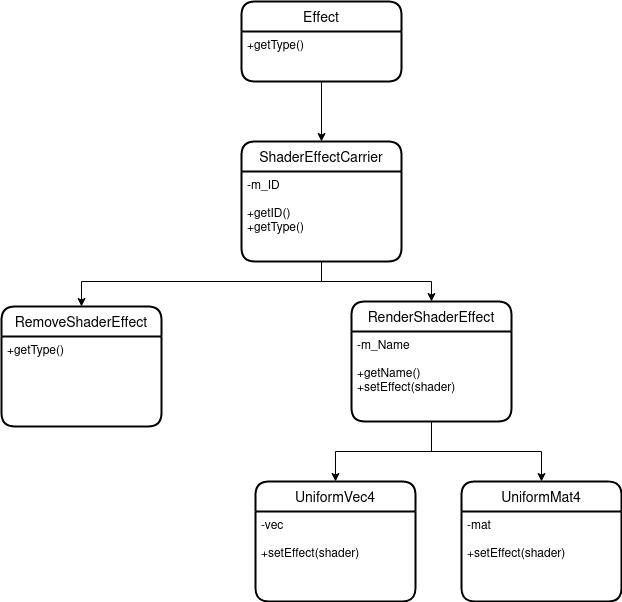
\includegraphics[scale=0.5]{img/Classes/Effects.png}}
                    \caption{Effect subclasses}
                    \label{fig}
                \end{figure}
                Effect
                \begin{center}
                    Functions
                    \begin{tabular}{ | m{0.15\textwidth} | m{0.35\textwidth}| m{0.4\textwidth} | }
                        \hline
                        \textbf{Function Name} & \textbf{Parameters} & \textbf{Description} \\
                        \hline
                        getType & & Returns the type of the effect \\
                        \hline
                    \end{tabular}
                \end{center}
                ShaderEffectCarrier
                \begin{center}
                    Variables
                    \begin{tabular}{ | m{0.45\textwidth} | m{0.45\textwidth} | }
                        \hline
                        \textbf{Variable Name} & \textbf{Description} \\
                        \hline
                        m\_ID & Stores the ID of the effect \\
                        \hline
                    \end{tabular}
                    Functions
                    \begin{tabular}{ | m{0.15\textwidth} | m{0.35\textwidth}| m{0.4\textwidth} | }
                        \hline
                        \textbf{Function Name} & \textbf{Parameters} & \textbf{Description} \\
                        \hline
                        getID & & Returns the ID of the effect \\
                        \hline
                    \end{tabular}
                \end{center}
                RemoveShaderEffect - Inherits everything from parent classes and only overrides \\
                ShaderEffect
                \begin{center}
                    Variables
                    \begin{tabular}{ | m{0.45\textwidth} | m{0.45\textwidth} | }
                        \hline
                        \textbf{Variable Name} & \textbf{Description} \\
                        \hline
                        m\_Name & Stores the name of the variable \\
                        \hline
                    \end{tabular}
                    Functions
                    \begin{tabular}{ | m{0.15\textwidth} | m{0.35\textwidth}| m{0.4\textwidth} | }
                        \hline
                        \textbf{Function Name} & \textbf{Parameters} & \textbf{Description} \\
                        \hline
                        getName & & Returns the name of the variable \\
                        \hline
                        setEffect & shader to set the effect to & Sets the current effect to the shader given \\
                        \hline
                    \end{tabular}
                \end{center}
                UniformVec4
                \begin{center}
                    Variables
                    \begin{tabular}{ | m{0.45\textwidth} | m{0.45\textwidth} | }
                        \hline
                        \textbf{Variable Name} & \textbf{Description} \\
                        \hline
                        vec & Stores the vector that is passed into the shader \\
                        \hline
                    \end{tabular}
                \end{center}
                UniformMat4
                \begin{center}
                    Variables
                    \begin{tabular}{ | m{0.45\textwidth} | m{0.45\textwidth} | }
                        \hline
                        \textbf{Variable Name} & \textbf{Description} \\
                        \hline
                        mat & Stores the matrix that is passed into the shader \\
                        \hline
                    \end{tabular}
                \end{center}
            \clearpage
            \subsubsection{Events}
                \begin{figure}[hbt!]
                    \centerline{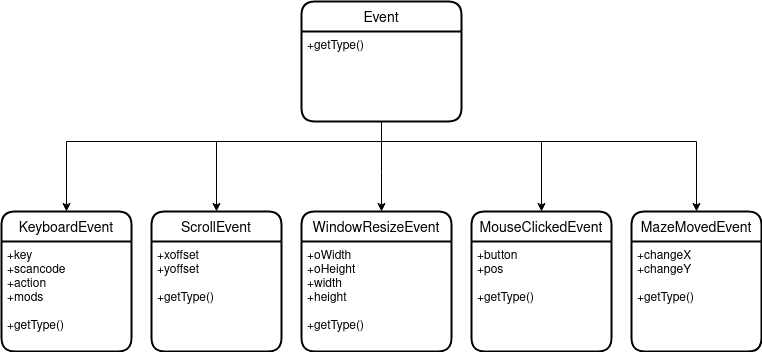
\includegraphics[scale=0.5]{img/Classes/Events.png}}
                    \caption{Event subclasses}
                    \label{fig}
                \end{figure}
                Event
                \begin{center}
                    Functions
                    \begin{tabular}{ | m{0.15\textwidth} | m{0.35\textwidth}| m{0.4\textwidth} | }
                        \hline
                        \textbf{Function Name} & \textbf{Parameters} & \textbf{Description} \\
                        \hline
                        getType & & Returns the type of event \\
                        \hline
                    \end{tabular}
                \end{center}
                keyboardEvent
                \begin{center}
                    Variables
                    \begin{tabular}{ | m{0.45\textwidth} | m{0.45\textwidth} | }
                        \hline
                        \textbf{Variable Name} & \textbf{Description} \\
                        \hline
                        key & Stores the key pressed \\
                        \hline
                        scancode & Stores the platform-specific scancode \\
                        \hline
                        action & Stores the action of the key (Release, press, hold)\\
                        \hline
                        mods & Stores the modifier bits \\
                        \hline
                    \end{tabular}
                \end{center}
                ScrollEvent
                \begin{center}
                    Variables
                    \begin{tabular}{ | m{0.45\textwidth} | m{0.45\textwidth} | }
                        \hline
                        \textbf{Variable Name} & \textbf{Description} \\
                        \hline
                        xoffset & Stores the change in the x direction \\
                        \hline
                        yoffset & Stores the change in the y direction \\
                        \hline
                    \end{tabular}
                \end{center}
                WindowResizeEvent
                \begin{center}
                    Variables
                    \begin{tabular}{ | m{0.45\textwidth} | m{0.45\textwidth} | }
                        \hline
                        \textbf{Variable Name} & \textbf{Description} \\
                        \hline
                        oWidth & Stores the width before the transformation \\
                        \hline
                        oHeight & Stores the height before the transformation \\
                        \hline
                        width & Stores the new width \\
                        \hline
                        height & Stores the new height \\
                        \hline
                    \end{tabular}
                \end{center}
                MouseClickedEvent
                \begin{center}
                    Variables
                    \begin{tabular}{ | m{0.45\textwidth} | m{0.45\textwidth} | }
                        \hline
                        \textbf{Variable Name} & \textbf{Description} \\
                        \hline
                        button & Stores the button that has been pressed \\
                        \hline
                        pos & Stores the position of the mouse \\
                        \hline
                    \end{tabular}
                \end{center}
                MazeMovedEvent
                \begin{center}
                    Variables
                    \begin{tabular}{ | m{0.45\textwidth} | m{0.45\textwidth} | }
                        \hline
                        \textbf{Variable Name} & \textbf{Description} \\
                        \hline
                        changeX & Stores the change in X that has happened \\
                        \hline
                        changeY & Stores the change in Y that has happened \\
                        \hline
                    \end{tabular}
                \end{center}
            \clearpage
            \subsubsection{Other}
                \begin{figure}[hbt!]
                    \centerline{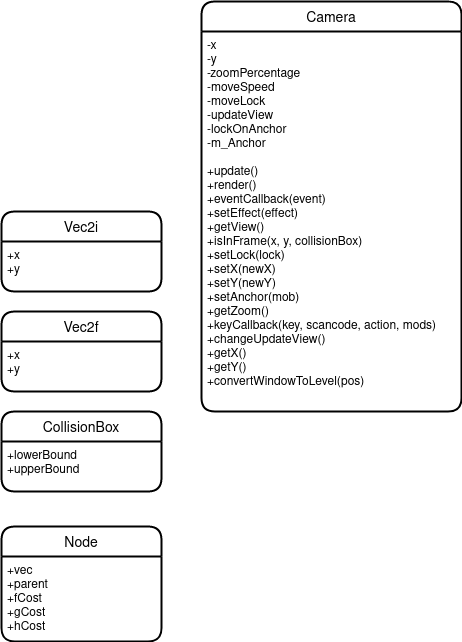
\includegraphics[scale=0.5]{img/Classes/Other.png}}
                    \caption{Classes that are for general use}
                    \label{fig}
                \end{figure}
                Camera
                \begin{center}
                    Variables
                    \begin{tabular}{ | m{0.45\textwidth} | m{0.45\textwidth} | }
                        \hline
                        \textbf{Variable Name} & \textbf{Description} \\
                        \hline
                        x & Stores x position of the camera \\
                        \hline
                        y & Stores the y position of the camera \\
                        \hline
                        zoomPercentage & Stores the zoom percentage of the objects \\
                        \hline
                        moveSpeed & Stores the speed it can move when disconnected from its anchor \\
                        \hline
                        moveLock & Stores whether it can move or not \\
                        \hline
                        updateView & Stores whether the view effect needs to be updated \\
                        \hline
                        lockOnAnchor & Stores whether it needs to be locked on its anchor \\
                        \hline
                        m\_Anchor & Stores the entity it is locked onto \\
                        \hline
                    \end{tabular}
                    Functions
                    \begin{tabular}{ | m{0.2\textwidth} | m{0.3\textwidth}| m{0.4\textwidth} | }
                        \hline
                        \textbf{Function Name} & \textbf{Parameters} & \textbf{Description} \\
                        \hline
                        update & & Updates the camera position \\
                        \hline
                        render & & Updates the view effect \\
                        \hline
                        eventCallback & event & Deals with current event \\
                        \hline
                        setEffect & effect & Allows camera to receive an effect \\
                        \hline
                        getView & & Returns the view matrix \\
                        \hline
                        isInFrame & Position and collision box & Returns whether it will be displayed onscreen \\
                        \hline
                        setLock & lock & Sets the lock \\
                        \hline
                        setX & new x coord & sets the x value \\
                        \hline
                        setY & new y coord & sets the y value \\
                        \hline
                        setAnchor & mob & Sets the anchor  \\
                        \hline
                        getZoom & & Returns the zoom \\
                        \hline
                        keyCallback & information stored in key event & Deals with a key being pressed \\
                        \hline
                        changeUpdateView & & changes the updateView variable to true so the view will be updated next render cycle \\
                        \hline
                        getX & & Returns the x value \\
                        \hline
                        getY & & Returns the y value \\
                        \hline
                        convertWindowToLevel & Position vector & Converts the position into coordinates in the level \\
                        \hline
                    \end{tabular}
                \end{center}
                Vec2i
                \begin{center}
                    Variables
                    \begin{tabular}{ | m{0.45\textwidth} | m{0.45\textwidth} | }
                        \hline
                        \textbf{Variable Name} & \textbf{Description} \\
                        \hline
                        x & Stores x position as an int \\
                        \hline
                        y & Stores y position as an int \\
                        \hline
                    \end{tabular}
                \end{center}
                Vec2f
                \begin{center}
                    Variables
                    \begin{tabular}{ | m{0.45\textwidth} | m{0.45\textwidth} | }
                        \hline
                        \textbf{Variable Name} & \textbf{Description} \\
                        \hline
                        x & Stores x position as an float \\
                        \hline
                        y & Stores y position as an float \\
                        \hline
                    \end{tabular}
                \end{center}
                CollisionBox
                \begin{center}
                    Variables
                    \begin{tabular}{ | m{0.45\textwidth} | m{0.45\textwidth} | }
                        \hline
                        \textbf{Variable Name} & \textbf{Description} \\
                        \hline
                        lowerBound & Stores the position of the bottom left corner (relative to the objects coordinates) \\
                        \hline
                        upperBound & Stores the position of the top right corner (relative to the objects coordinates) \\
                        \hline
                    \end{tabular}
                \end{center}
                Node
                \begin{center}
                    Variables
                    \begin{tabular}{ | m{0.45\textwidth} | m{0.45\textwidth} | }
                        \hline
                        \textbf{Variable Name} & \textbf{Description} \\
                        \hline
                        vec & Stores the position of the node (as integer in the grid) \\
                        \hline
                        parent & Stores the parent (as a position on the grid) \\
                        \hline
                        fCost & The total cost of the node \\
                        \hline
                        gCost & The distance from the start node \\
                        \hline
                        hCost & The distance from the destination node \\
                        \hline
                    \end{tabular}
                \end{center}
            \clearpage
        \subsection{Functions}
            \subsubsection{Control}
            \begin{center}
                \begin{tabular}{ | m{0.15\textwidth} | m{0.35\textwidth}| m{0.4\textwidth} | }
                    \hline
                    \textbf{Function Name} & \textbf{Parameters} & \textbf{Description} \\
                    \hline
                    main & & First function that is run when the program boots up \\
                    \hline
                    gameLoop & & Function that controls the game loop and tells the application when to render and update \\
                    \hline
                    & & \\
                    \hline
                \end{tabular}
            \end{center}
            \subsubsection{Utils}
            \begin{center}
                \begin{tabular}{ | m{0.2\textwidth} | m{0.3\textwidth}| m{0.4\textwidth} | }
                    \hline
                    \textbf{Function Name} & \textbf{Parameters} & \textbf{Description} \\
                    \hline
                    getIndexOfInsertion & Array which the element will be added to, nodeMap and the next node & Uses binomial search to find the position of where to insert a new element \\
                    \hline
                    factorial & num & Returns the result of a factorial \\
                    \hline
                    directionToRotation & direction & Converts a direction into radians \\
                    \hline
                    distanceBetweenVec2i & start and end positions & Calculates the distance between two vectors using pythagoras \\
                    \hline
                    distanceBetweenVec2f & start and end positions &  Calculates the distance between two vectors using pythagoras\\
                    \hline
                    & & \\
                    \hline
                \end{tabular}
            \end{center}
\end{document}